% Pre-ambulo
\documentclass[
  % -- opções da classe memoir --
  12pt,                 % tamanho da fonte
  openright,            % capítulos começam em pág ímpar (insere página vazia caso preciso)
  twoside,              % para impressão em recto e verso. Oposto a oneside
  a4paper,              % tamanho do papel.
  % -- opções da classe abntex2 --
  sumario=abnt-6027-2012,
  chapter=TITLE,        % títulos de capítulos convertidos em letras maiúsculas
  section=TITLE,        % títulos de seções convertidos em letras maiúsculas
  %subsection=TITLE,    % títulos de subseções convertidos em letras maiúsculas
  %subsubsection=TITLE, % títulos de subsubseções convertidos em letras maiúsculas
  % -- opções do pacote babel --
  english,              % idioma adicional para hifenização
  french,               % idioma adicional para hifenização
  spanish,              % idioma adicional para hifenização
  brazil                % o último idioma é o principal do documento
]{abntex2}

% ---
% Pacotes básicos
% ---

\usepackage{lmodern}        % Usa a fonte Latin Modern
\usepackage{times}          % Usa a fonte Times New Roman
\usepackage[T1]{fontenc}    % Selecao de codigos de fonte.
\usepackage[utf8]{inputenx} % Codificacao do documento (conversão automática dos acentos)
\usepackage{indentfirst}    % Indenta o primeiro parágrafo de cada seção.
\usepackage{color}          % Controle das cores
\usepackage{graphicx}       % Inclusão de gráficos
\usepackage{microtype}      % para melhorias de justificação
% \usepackage[brazil]{babel}
\usepackage[boxed,vlined,linesnumbered,portuguese,portuguesekw]{algorithm2e-mod}
% ---

% ---
% Pacotes de citações
% ---
\usepackage[brazilian,hyperpageref]{backref}   % Paginas com as citações na bibl
\usepackage[alf,abnt-emphasize=bf]{abntex2cite}  % Citações padrão ABNT

% ---
% CONFIGURAÇÕES DE PACOTES
% ---

% ---
% Configurações do pacote backref
% Usado sem a opção hyperpageref de backref
%\renewcommand{\backrefpagesname}{Citado na(s) página(s):~}
\renewcommand{\backrefpagesname}{}
% Texto padrão antes do número das páginas
\renewcommand{\backref}{}
% Define os textos da citação
% \renewcommand*{\backrefalt}[4]{
%   \ifcase #1 %
%     Nenhuma citação no texto.%
%   \or
%     Citado na página #2.%
%   \else
%     Citado #1 vezes nas páginas #2.%
%   \fi}%
\renewcommand*{\backrefalt}[4]{}
% ---

\usepackage{textcase}
\usepackage[useregional]{datetime2}
\usepackage{datetime2-calc}
\usepackage[normalem]{ulem}

\usepackage[hypcap=true,justification=centering,skip=0cm]{caption}
\usepackage[justification=centering,skip=0cm]{subcaption}

% \usepackage{newpxtext}
\captionsetup[table]{skip=0cm}
\captionsetup[figure]{skip=0cm}
\captionsetup[subfigure]{skip=0cm}

\usepackage{hyphenat}
\usepackage{booktabs}
\usepackage{navigator}
\usepackage{listings}

% \usepackage{float}
\usepackage{multirow}
% \usepackage[all]{nowidow}

\usepackage{mdframed}

% \setfloatlocations{figure}{!htb}
\setfloatlocations{figure}{!hbtp}
\setfloatlocations{table}{!hbtp}

\graphicspath{ {./imagens/} }

\usepackage{enumitem}
% \setlist{itemsep=4pt,parsep=4pt,topsep=8pt,partopsep=4pt}
% \setlist{nosep}

% \floatstyle{boxed}
% \restylefloat{figure}

\usepackage[dvipsnames]{xcolor}

\definecolor{tamarillo}{RGB}{163,20,20}
\definecolor{brightturquoise}{rgb}{0.03, 0.91, 0.87}
\definecolor{malachite}{rgb}{0.04, 0.85, 0.32}

% Redefinição de instruções

\providecommand{\tightlist}{%
  \setlength{\itemsep}{0pt}\setlength{\parskip}{0pt}
}

% \renewcommand{\listingscaption}{Fig.}
% \renewcommand\theFancyVerbLine{\rm{\arabic{FancyVerbLine}}}

% -----
% Declarações de cabecalhos
% -----
% Cabecalho padrao
\makepagestyle{abntbookheadings}
% \makeevenhead{abntbookheadings}{\ABNTEXfontereduzida\thepage}{}{}
\makeevenhead{abntbookheadings}{}{}{\ABNTEXfontereduzida\thepage}
\makeoddhead{abntbookheadings}{}{}{\ABNTEXfontereduzida\thepage}
%\makeheadrule{abntbookheadings}{\textwidth}{\normalrulethickness}

% Cabecalho do inicio do capitulo
\makepagestyle{abntbookchapfirst}
\makeoddhead{abntbookchapfirst}{}{}{\ABNTEXfontereduzida\thepage}

% Configura layout para elementos textuais
\renewcommand{\textual}{%
  \pagestyle{abntbookheadings}%
  \aliaspagestyle{chapter}{abntbookchapfirst}% customizing chapter pagestyle
  %\nouppercaseheads%
  \bookmarksetup{startatroot}%
}
% ---

\DTMsavedate{mdate}{2018-12-07}
\date{\DTMusedate{mdate}}

\title{Um Modelo Espaço-Temporal para Explorar Regiões Densas Interessantes}
\author{Felipe Mateus Freire Pontes}
\local{\uppercase{Natal}}
\date{2018}
\orientador{Plácido Antônio da Silva Neto}
\newcommand{\examinadorA}{Jorgiano Márcio Bruno Vidal}
\newcommand{\examinadorB}{Marília Aranha Freire}
\instituicao{%
  Instituto Federal do Rio Grande do Norte -- IFRN
  \par
  Diretoria de Gestão e Tecnologia da Informação -- DIATINF
  \par
  Curso de Tecnologia em Análise e Desenvolvimento de Sistemas -- TADS
}
\tipotrabalho{TCC (Graduação)}
% O preambulo deve conter o tipo do trabalho, o objetivo,
% o nome da instituição e a área de concentração
\preambulo{%
Trabalho de conclusão de curso apresentado ao Curso Superior de Tecnologia em Análise e Desenvolvimento de Sistemas da Diretoria Acadêmica de Gestão e Tecnologia da Informação do Instituto Federal de Educação, Ciência e Tecnologia do Rio Grande do Norte como requisito parcial à obtenção do título de Tecnólogo em Análise e Desenvolvimento de Sistemas.
}

\makeatletter
\hypersetup{
  pdftitle={\@title},
  pdfauthor={\@author},
  pdfsubject={\imprimirpreambulo},
  pdfkeywords={Dados Espaciais}{Análise Temporal}{Preferência do Usuário},
  pdfcreator={LaTeX with abnTeX2},
  colorlinks=false,
  % linkcolor=blue,
  % citecolor=blue,
  % urlcolor=blue
}
\makeatother

% ---
% Possibilita criação de Quadros e Lista de quadros.
% Ver https://github.com/abntex/abntex2/issues/176
%
\newcommand{\quadroname}{Quadro}
\newcommand{\listofquadrosname}{Lista de quadros}

\newfloat{quadro}{loq}{\quadroname}
\newlistof{listofquadros}{loq}{\listofquadrosname}
\newlistentry{quadro}{loq}{0}

% configurações para atender às regras da ABNT
\setfloatadjustment{quadro}{\centering}
\counterwithout{quadro}{chapter}
\renewcommand{\cftquadroname}{\quadroname\space}
\renewcommand*{\cftquadroaftersnum}{\hfill--\hfill}

\setfloatlocations{quadro}{!hbtp}

\makeatletter
\renewcommand*{\ext@quadro}{lof}
\makeatother
% ---

% ---
% Posiciona figuras e tabelas no topo da página quando adicionadas sozinhas
% em um página em branco. Ver https://github.com/abntex/abntex2/issues/170
\makeatletter
\setlength{\@fptop}{5pt} % Set distance from top of page to first float
\makeatother
% ---

\renewcommand{\fontename}{Fonte}
\renewcommand{\ABNTEXcaptionfontedelim}{:}

\makeatletter
\renewcommand{\fonte}[2][\fontename]{%
  \memlegendinfo{#2}%
  \par
\begingroup
    \ABNTEXfontereduzida
    \configureseparator
    \captiondelim{:~}
    \@makecaption{\ABNTEXfontereduzida #1}{\ignorespaces\ABNTEXfontereduzida #2}\par
\endgroup}
\makeatother

\newcommand{\mfonte}[0]{%
  \fonte{Elaboração própria em \DTMfetchyear{mdate}}}

\newcommand{\mcaption}[1]
{%
  \caption[#1]{%
    #1
  }
}

\mdfsetup{
  leftmargin=0cm,
  skipabove=0cm,
  rightmargin=0cm,
  skipbelow=0cm,
  innertopmargin=.1cm,
  innerrightmargin=.1cm,
  innerleftmargin=.1cm,
  innerbottommargin=.1cm,
}

\newlength{\MaxSizeOfLineNumbers}%
% Adjust to maximum number of lines
\settowidth{\MaxSizeOfLineNumbers}{99}%
\addtolength{\MaxSizeOfLineNumbers}{2.5ex}%
\lstset{
  showstringspaces=false,
  numbers=left,
  numbersep=2.5ex,
  xleftmargin=\MaxSizeOfLineNumbers,
  keywordstyle=\color{blue},
  basicstyle=\ttfamily,
  breaklines=true,
  stringstyle=\color{tamarillo},
  literate=
    {á}{{\'a}}1
    {à}{{\`a}}1
    {é}{{\'e}}1
    {ê}{{\^e}}1
    {ã}{{\~a}}1
    {ó}{{\'o}}1
    {ç}{{\c{c}}}1%
}
\renewcommand\sout[1]{}
\usepackage[export]{adjustbox}

\let\oldincludegraphics\includegraphics
\renewcommand{\includegraphics}[2][]{%
%   \begin{mdframed}%
%   \begin{center}%
    \centering%
    \oldincludegraphics[max width=.7\linewidth,#1]{#2}%
%   \end{center}%
%   \end{mdframed}%
}

\setlength{\ABNTEXsignwidth}{10cm}

% ---
% Espaçamentos entre linhas e parágrafos
% ---

% O tamanho do parágrafo é dado por:
\setlength{\parindent}{1.3cm}

% Controle do espaçamento entre um parágrafo e outro:
\setlength{\parskip}{0.2cm}  % tente também \onelineskip

% \renewcommand{\ABNTEXchapterfont}{\bfseries}
% \newcommand{\ABNTEXpartfont}{\ABNTEXchapterfont}
%
% Fontes das entradas do sumario
%
% \renewcommand{\cftpartfont}{\bfseries\larger}

\renewcommand*{\cftchapterleader}{\hfill}
\renewcommand*{\cftsectionleader}{\hfill}
\renewcommand*{\cftsubsectionleader}{\hfill}
\renewcommand*{\cftsubsubsectionleader}{\hfill}
\renewcommand*{\cftparagraphleader}{\hfill}

\setlength{\cftbeforechapterskip}{0em}

%--
% seção primária
%--
\renewcommand{\cftchapterfont}{\bfseries}
\renewcommand{\cftchapterpagefont}{\normalsize\normalfont}
%--
% seção secundária
%--
\renewcommand{\cftsectionfont}{\normalfont}
\renewcommand{\cftsectionpagefont}{\normalsize\normalfont}
%--
% seção terciária
%--
\renewcommand{\cftsubsectionfont}{\normalfont\bfseries}
\renewcommand{\cftsubsectionpagefont}{\normalsize\normalfont}
%--
% seção quaternária
%--
\renewcommand{\cftsubsubsectionfont}{\normalfont}
\renewcommand{\cftsubsubsectionpagefont}{\normalsize\normalfont}
%--
% seção quinária
%--
\renewcommand{\cftparagraphfont}{\normalfont\itshape}
\renewcommand{\cftparagraphpagefont}{\normalsize\normalfont}

\makeatletter
\let\oldcontentsline\contentsline
\def\contentsline#1#2{%
  \expandafter\ifx\csname l@#1\endcsname\l@section
  \expandafter\@firstoftwo
  \else
  \expandafter\@secondoftwo
  \fi
  {%
    \oldcontentsline{#1}{\MakeTextUppercase{#2}}%
  }{%
  \oldcontentsline{#1}{#2}%
}%
}
\makeatother

% \renewcommand{\cftsubsectionfont}{\bfseries}
% \renewcommand{\cftsubsectionpagefont}{\normalsize\cftsubsectionfont}

% \renewcommand{\cftsubsubsectionfont}{\normalsize}
% \renewcommand{\cftsubsubsectionpagefont}{\cftsubsubsectionfont}

% \renewcommand{\cftparagraphfont}{\footnotesize}
% \renewcommand{\cftparagraphpagefont}{\cftparagraphfont}

%
% Fontes das seções/capítulos
%
\renewcommand{\ABNTEXpartfontsize}{\normalsize}

\renewcommand{\ABNTEXchapterfont}{\bfseries}
\renewcommand{\ABNTEXchapterfontsize}{\normalsize}

\renewcommand{\ABNTEXsectionfont}{\normalsize}
\renewcommand{\ABNTEXsectionfontsize}{\normalsize}

\renewcommand{\ABNTEXsubsectionfont}{\bfseries}
\renewcommand{\ABNTEXsubsectionfontsize}{\normalsize}

\renewcommand{\ABNTEXsubsubsectionfontsize}{\normalfont}
\renewcommand{\ABNTEXsubsubsubsectionfontsize}{\normalfont\itshape}

% \newcommand{\ABNTEXsectionfont}{\ABNTEXchapterfont}
% \newcommand{\ABNTEXsubsectionfont}{\ABNTEXsectionfont}
% \newcommand{\ABNTEXsubsubsectionfont}{\ABNTEXsubsectionfont}
% \newcommand{\ABNTEXsubsubsubsectionfont}{\ABNTEXsubsectionfont}

% ---
% compila o indice
% ---
\makeindex

% \setlength{\parindent}{1pt}
\setlength{\parskip}{0pt}

\setlength{\beforechapskip}{1.0\onelineskip}
\setlength{\afterchapskip}{1.0\onelineskip}

\setlength{\beforesecskip}{1.0\onelineskip}
\setlength{\aftersecskip}{1.0\onelineskip}

\setlength{\beforesubsecskip}{1.0\onelineskip}
\setlength{\aftersubsecskip}{1.0\onelineskip}

\setlength{\textfloatsep}{1.0\onelineskip}
\setlength{\floatsep}{1.0\onelineskip}
\setlength{\intextsep}{1.0\onelineskip}


% Definicao da lista de simbolos
% \simb[entrada na lista de simbolos]{simbolo}:
% Escreve o simbolo no texto e uma entrada na lista de simbolos.
% Se o parametro opcional e omitido, usa-se o parametro obrigatorio.
\newcommand{\simb}[2][]
{%
	\ifthenelse{\equal{#1}{}}
	{\addcontentsline{los}{simbolo}{#2}}
	{\addcontentsline{los}{simbolo}{#1}}#2
}
% Para aceitar comandos com @ (at) no nome
\makeatletter 
% \listadesimbolos: comando que imprime a lista de simbolos
\newcommand{\listadesimbolos}
{
	\pretextualchapter{Lista de símbolos}
	{\setlength{\parindent}{0cm}
  \@starttoc{los}}  
}
% Como a entrada sera impressa
\newcommand\l@simbolo[2]{\par #1}
\makeatother


% Definicao da lista de abreviaturas e siglas
% \abrv[entrada na lista de simbolos]{abreviatura}:
% Escreve a sigla/abreviatura no texto e uma entrada na lista de abreviaturas e siglas.
% Se o parametro opcional e omitido, usa-se o parametro obrigatorio.
\newcommand{\abrv}[2]
{%
	% \ifthenelse{\equal{#1}{}}
	% {\addcontentsline{loab}{abreviatura}{#2}}
	{\addcontentsline{loab}{abreviatura}{#1 #2}}{#1}}
% Para aceitar comandos com @ (at) no nome
\makeatletter 
% \listadeabreviaturas: comando que imprime a lista de abreviaturas e siglas
\newcommand{\listadeabreviaturas}
{
  % \pretextualchapter{Lista de abreviaturas e siglas}
  \begin{siglas}
    \@OnehalfSpacing
    % % {\setlength{\parindent}{0cm}
    \item[IDR] \textit{Interesting Dense Region}
    \item[IFRN] Instituto Federal do Rio Grande do Norte
    \item[TADS] Tecnologia em Análise e Desenvolvimento de Sistemas
    % \@starttoc{loab}
  \end{siglas}
	% {\setlength{\parindent}{0cm}
  % }
}
% Como a entrada sera impressa
\newcommand\l@abreviatura[2]{\par #1}
\makeatother


% \listofalgorithms: comando que imprime a lista de algoritmos
% \renewcommand{\listalgorithmname}{Lista de algoritmos}


\newcommand{\myThesis}{Um Modelo Espaço-Temporal para Explorar Regiões Densas Interessantes}
\newcommand{\myThesisEnglish}{An Spatial-Temporal Model for Exploring Interesting Dense Regions}
\newcommand{\myName}{Felipe Mateus Freire Pontes}
\newcommand{\mySupervisorName}{Dr. Plácido Antônio de Souza Neto}
\newcommand{\myFirstExaminerName}{Dr. Jorgiano Márcio Bruno Vidal}
\newcommand{\mySecondExaminerName}{Dra. Marília Aranha Freire}
\newcommand{\myDeriveryDate}{Dezembro, 2018}
\newcommand{\myDefenseDate}{07 de dezembro de 2018}
\newcommand{\myLineOfResearch}{Banco de Dados, Análise de Dados}

\newcommand{\todo}[1]{}
\newcommand{\closesubsection}{
	\vspace{25pt}
	\noindent
}

\begin{document}
  \selectlanguage{brazil}
  \frenchspacing

  \frontmatter

  % Capa
% Prote��o externa do trabalho e sobre a qual se imprimem as informa��es indispens�veis 
% � sua identifica��o.

% Especifica��o da capa
\begin{titlepage}
	\begin{center}
		
		  
		\begin{minipage}{11.15cm}
			\begin{center}
				\begin{espacosimples}
					{\small \ \\
                       \textsc{Instituto Federal do Rio Grande do Norte}
                       \\
							  \textsc{Campus Natal - Central}					\\
							  \textsc{Diretoria de Gestão e Tecnologia da Informação}	   
							  \\
							  \textsc{Tecnologia em Análise e Desenvolvimento de Sistemas}}   	
                       \\
				\end{espacosimples}
			\end{center}
		\end{minipage}

			
		\vspace{6cm}
						
		% T�tulo do trabalho
		{\setlength{\baselineskip}%
		{1.3\baselineskip}
		{\LARGE \textbf{Título do trabalho}}\par}
			
		\vspace{3cm}
			
		% Nome do aluno (autor)
		{\large \textbf{Nome completo do autor}}
						
		\vspace{6cm}
		
		% Local da institui��o onde o trabalho deve ser apresentado e ano de entrega do mesmo
		Natal-RN\\Mês (por extenso) e ano
	\end{center}
\end{titlepage}
  % Folha de rosto
% Cont�m os elementos essenciais � identificação do trabalho.

% T�tulo, nome do aluno e respectivo orientador e filiação
\titulo{\Large{Implementação e Análise de Algoritmos para Solução do Cubo de Rubik}}
\autor{Camila Jordana Ribeiro Teixeira}
\orientador[Orientador]{\par Prof. Dr. Plácido Antônio de Souza Neto}
\instituicao
{
   TADS -- Curso de Tecnologia em Análise e Desenvolvimento de
   Sistemas\par 
   DIATINF -- Diretoria Acadêmica de gestão e Tecnologia da Informação\par 
   CNAT -- Campus Natal - Central\par 
   IFRN -- Instituto Federal do Rio Grande do Norte }
	
% Natureza do trabalho (não deve ser modificada)
\comentario
{
	Trabalho de conclusão de curso de graduação do curso de Tecnologia em Análise e
	Desenvolvimento de Sistemas da Diretoria de Gestão e Tecnologia de Informação
	do Instituto Federal do Rio Grande do Norte como requisito parcial para a
	obtenção do grau de Tecnólogo em Análise e Desenvolvimento de
	Sistemas.\bigskip\\
   \textit{Linha de pesquisa}:\\Análise de Algoritmos
}
		
% Local e data
\local{Natal-RN}
\data{Dezembro - 2017}
	
\folhaderosto

  % Folha de aprova��o
\begin{folhadeaprovacao}
	\setlength{\ABNTsignthickness}{0.4pt}
	\setlength{\ABNTsignwidth}{10cm}
	
	\noindent 
	Trabalho de Conclusão de Curso de Graduação sob o título
	\textit{Título} apresentada por Nome completo do autor e aceita pelo Diretoria
	de Gestão e Tecnologia da Informação do Instituto Federal do Rio Grande do
	Norte, sendo aprovada por todos os membros da banca examinadora abaixo especificada:
		
	% Membros da banca examinadora e respectivas filia��es
	\assinatura
	{
		Nome completo do orientador e titulação   			                  \\
		{\small Presidente}											          \smallskip\\ 
		{\footnotesize
			DIATINF -- Diretoria Acadêmica de Gestão e Tecnologia da Informação		   \\
		  	IFRN -- Instituto Federal do Rio Grande do Norte
		}
   }
      
   \assinatura
	{
      Nome completo do examinador e titulação   			                  \\
		{\small Examinador}											          \smallskip\\ 
		{\footnotesize
			Diretoria/Departamento		\\
		  	Instituto
		}
   }   
   
   \assinatura
	{
      Nome completo do examinador e titulação   			                  \\
		{\small Examinador}											          \smallskip\\ 
		{\footnotesize
			Diretoria/Departamento		\\
		  	Universidade
		}
	}
		
	\vfill
	
	\begin{center}
		Natal-RN, data da defesa (dia, mês e ano).
	\end{center}
\end{folhadeaprovacao}

  % Dedicat�ria


% \vspace{15cm}
% \begin{flushright}
	
% \end{flushright}


\begin{dedicatoria}
	\vspace*{\fill}
	\begin{flushright}
		Aos meus pais que nunca duvidaram de mim.
	\end{flushright}
	\vspace{4cm}
\end{dedicatoria}

  % Agradecimentos

\chapter*{Agradecimentos}

Ao meu orientador \mySupervisorName, pelo seu empenho em sempre buscar extrair o melhor de mim.

À Behrooz Omidvar-Tehrani, pelas suas colaborações mesmo estando a um oceano de distância.

À Francisco Bento da Silva Júnior, pelas suas contribuições como amigo e colega de pesquisa.

  % Ep�grafe (cita��o seguida de indica��o de autoria)

\chapter*{}
\vspace{15cm}
\begin{flushright}
	\textit
	{
		Se você for curioso, encontrará quebra-cabeças em torno de você. Se você estiver determinado, irá resolvê-los.
	}\medskip\\ 
	Erno Rubik
\end{flushright}

  % Resumo
\begin{center}
	{\Large{\textbf{\myThesis}}}
\end{center}

\vspace{1cm}

\begin{flushright}
	Autor: \myName\\
	Orientador(a): \mySupervisorName
\end{flushright}

\vspace{1cm}

\begin{center}
	\Large{\textsc{\textbf{Resumo}}}
\end{center}

\noindent O resumo deve apresentar de forma concisa os pontos relevantes de um
texto, fornecendo uma visão rápida e clara do conteúdo e das conclusões do
trabalho. O texto, redigido na forma impessoal do verbo, é constituído de uma
sequência de frases concisas e objetivas e não de uma simples enumeração de
tópicos, não ultrapassando 500 palavras, seguido, logo abaixo, das palavras
representativas do conteúdo do trabalho, isto é, palavras-chave e/ou
descritores. Por fim, deve-se evitar, na redação do resumo, o uso de parágrafos
(em geral resumos são escritos em parágrafo único), bem como de fórmulas,
diagramas e símbolos, optando-se, quando necessário, pela transcrição na forma
extensa, além de não incluir citações bibliográficas.

\noindent\textit{Palavras-chave}: Palavra-chave 1, Palavra-chave 2, Palavra-chave 3.
  % Resumo em l�ngua estrangeira (em ingl�s Abstract, em espanhol Resumen, em franc�s R�sum�)
\begin{center}
	{\Large{\textbf{Sentiment analysis model to extract data from social network}}}
\end{center}

\vspace{1cm}

\begin{flushright}
	Author: Yuri Jordan de Melo Oliveira\\
	Supervisor: Prof. Plácido Antônio de Souza Neto, Ph.D.
\end{flushright}

\vspace{1cm}

\begin{center}
	\Large{\textsc{\textbf{Abstract}}}
\end{center}

\noindent Is noticed that, currently, the technical ability to collect, analyse and use information about humans`s opinions and thoughts, has its development boosted because of the spread of the social networks, to a world scale, these capabilities, have been applied for the understanding and decision-making, in the various areas of society such as health, education, politics and economy. An exploratory is made and a model for the analysis of textual data extracted from social networks is developed, in order to know if, what the users of these networks write in them, has a positive, neutral or negative feeling. To achieve this, it is necessary to generate a model for this type of analysis, implement the necessary algorithms for this purpose and a web service, in order to expose these algorithms and applying them in a case study, with some of the pre-candidates for the presidency of the Republic of Brazil, in 2018. It is then done, an exploratory research about. Therefore, 2470 messages were collected and analyzed, being classified as negative, neutral or positive and marked on a map, the place from which they came.

\noindent Keywords:  Sentiment analysis, Natural Language Processing, Social network.





  % ---
  % inserir lista de ilustrações
  % ---
  \pdfbookmark[0]{\listfigurename}{lof}
  \listoffigures*
  \cleardoublepage
  % ---

  % ---
  % inserir lista de tabelas
  % ---
  \pdfbookmark[0]{\listtablename}{lot}
  \listoftables*
  \cleardoublepage
  % ---

  % \listadeabreviaturas
  % \cleardoublepage

  % ---
  % inserir o sumario
  % ---
  \pdfbookmark[0]{\contentsname}{toc}
  \tableofcontents*
  \cleardoublepage
  % ---

  % Parte central do trabalho, englobando os capítulos que constituem o mesmo
  % Os referidos capítulos devem ser organizados dentro do diretório "Capítulos"

  \mainmatter

	\chapter{Introdução}
\label{chap:introducao}

Mais do que nunca estamos sobrecarregados com a quantidade de dados que criamos a cada dia. Quando comparamos quanto de informação vem sendo gerada nos ultimos anos, percebemos que está aumentando significamente. Além dessa evolução quantitativa, hoje temos os mais diversos tipos de informação, por exemplo: documentos, tuítes, fotos, vídeos, \textit{GIFs}, \textit{check-ins} entre vários outros.

Esse fenômeno vem sido chamado de \textit{Big Data} e representa uma crescente área de estudo atualmente. Como consequência, pesquisadores estão analisando e aprendendo com essas informações geradas, entretanto o crescimento contínuo da quantidade de dados dificulta as análises. Portanto pessoas estão investindo em novas técnicas e ferramentas para romper desafios como mineração de dados, {\em data cleaning}, visualização de dados, classificação de dados, exploração de dados e muito mais.

Um tipo comum de dados é o que chamamos de dado espacial, o qual a informação possui atributos geográficos como latitude e longitudade (por exemplo: tuítes, avaliação de restaurantes, {\em check-ins} em estabelecimentos). Dados espaciais podem ser muito significativo, por exemplo, um {\em check-in} no aeroporto por sua irmã na manhã do seu aniversário, provavelmente significa que você terá uma surpresa.

Cada registro em dados espaciais representa uma atividade numa precisa localização geográfica, em outras palavras, a análise desse tipo de dado permite realizar descobertas baseadas em fatos. Analistas estão frequetemente interessados em observar padrões espaciais e tendências para melhorar seus processos de tomada de decisão. Análise de dados espaciais tem várias aplicações como gerenciamento de cidade inteligentes, gerenciamento de disastres e transporte autônomo \cite{RoddickEHPS04,Telang:2012}.

\section{Problema}

A análise de dados espaciais geralmente é realizada num contexto exploratório: o analista não tem uma consulta precisa em mente e ele explora os dados em passos iterativos a fim de encontrar resultados potencialmente interessantes. Tradicionalmente, um cenário de análise exploratória é descrito na seguinte maneira: o analista visualiza um subconjunto de dados usando uma consulta em ambiente de visualização (por exemplo: Tableau\footnote{\it http://www.tableau.com},
Exhibit\footnote{\it http://www.simile-widgets.org/exhibit/},
Spotfire\footnote{\it http://spotfire.tibco.com}); o resultado será ilustrado em um mapa geográfico; então o analista investiga diferentes partes do conjuto de dados movendo ou focando o mapa afim de encontrar padrões ou tendências de interesse. O analista pode iterar por esse processo várias vezes realizando consultas diferentes e focando em diferentes aspectos.

Contudo, a vasto tamanho do conjunto de dados espacias faz com que o analista se sinta perdido durante a exploração. É possível ter milhares de pontos geográficos em cada bairro de uma cidade, por exemplo. Analistas precisam ter acesso apenas a algumas opções (chamadas de ``highlights'') que ajam como uma direção e assim permitir que ele foque no que lhe interessa na análise. No cenário perfeito, essas opções não são aleatoriamente escolhidas e representam o que o analista se mostrou interessado em iterações passadas.

Neste trabalho, formulamos uma solução para ``realçamento de dados usando feedback coletado ao longo do tempo''. Em outras palavras, buscamos realçar alguns pontos geográficos baseado nos interesses do analista afim de guiá-lo na direção ao que ele deve se concentrar nas iterações seguintes do processo de análise.

\subsection{Caso de Estudo}

Nessa seção, vamos apresentar um caso de estudo afim de demostrar a funcionalidade da nossa abordagem na prática.

\begin{figure}[t]
	\centering
	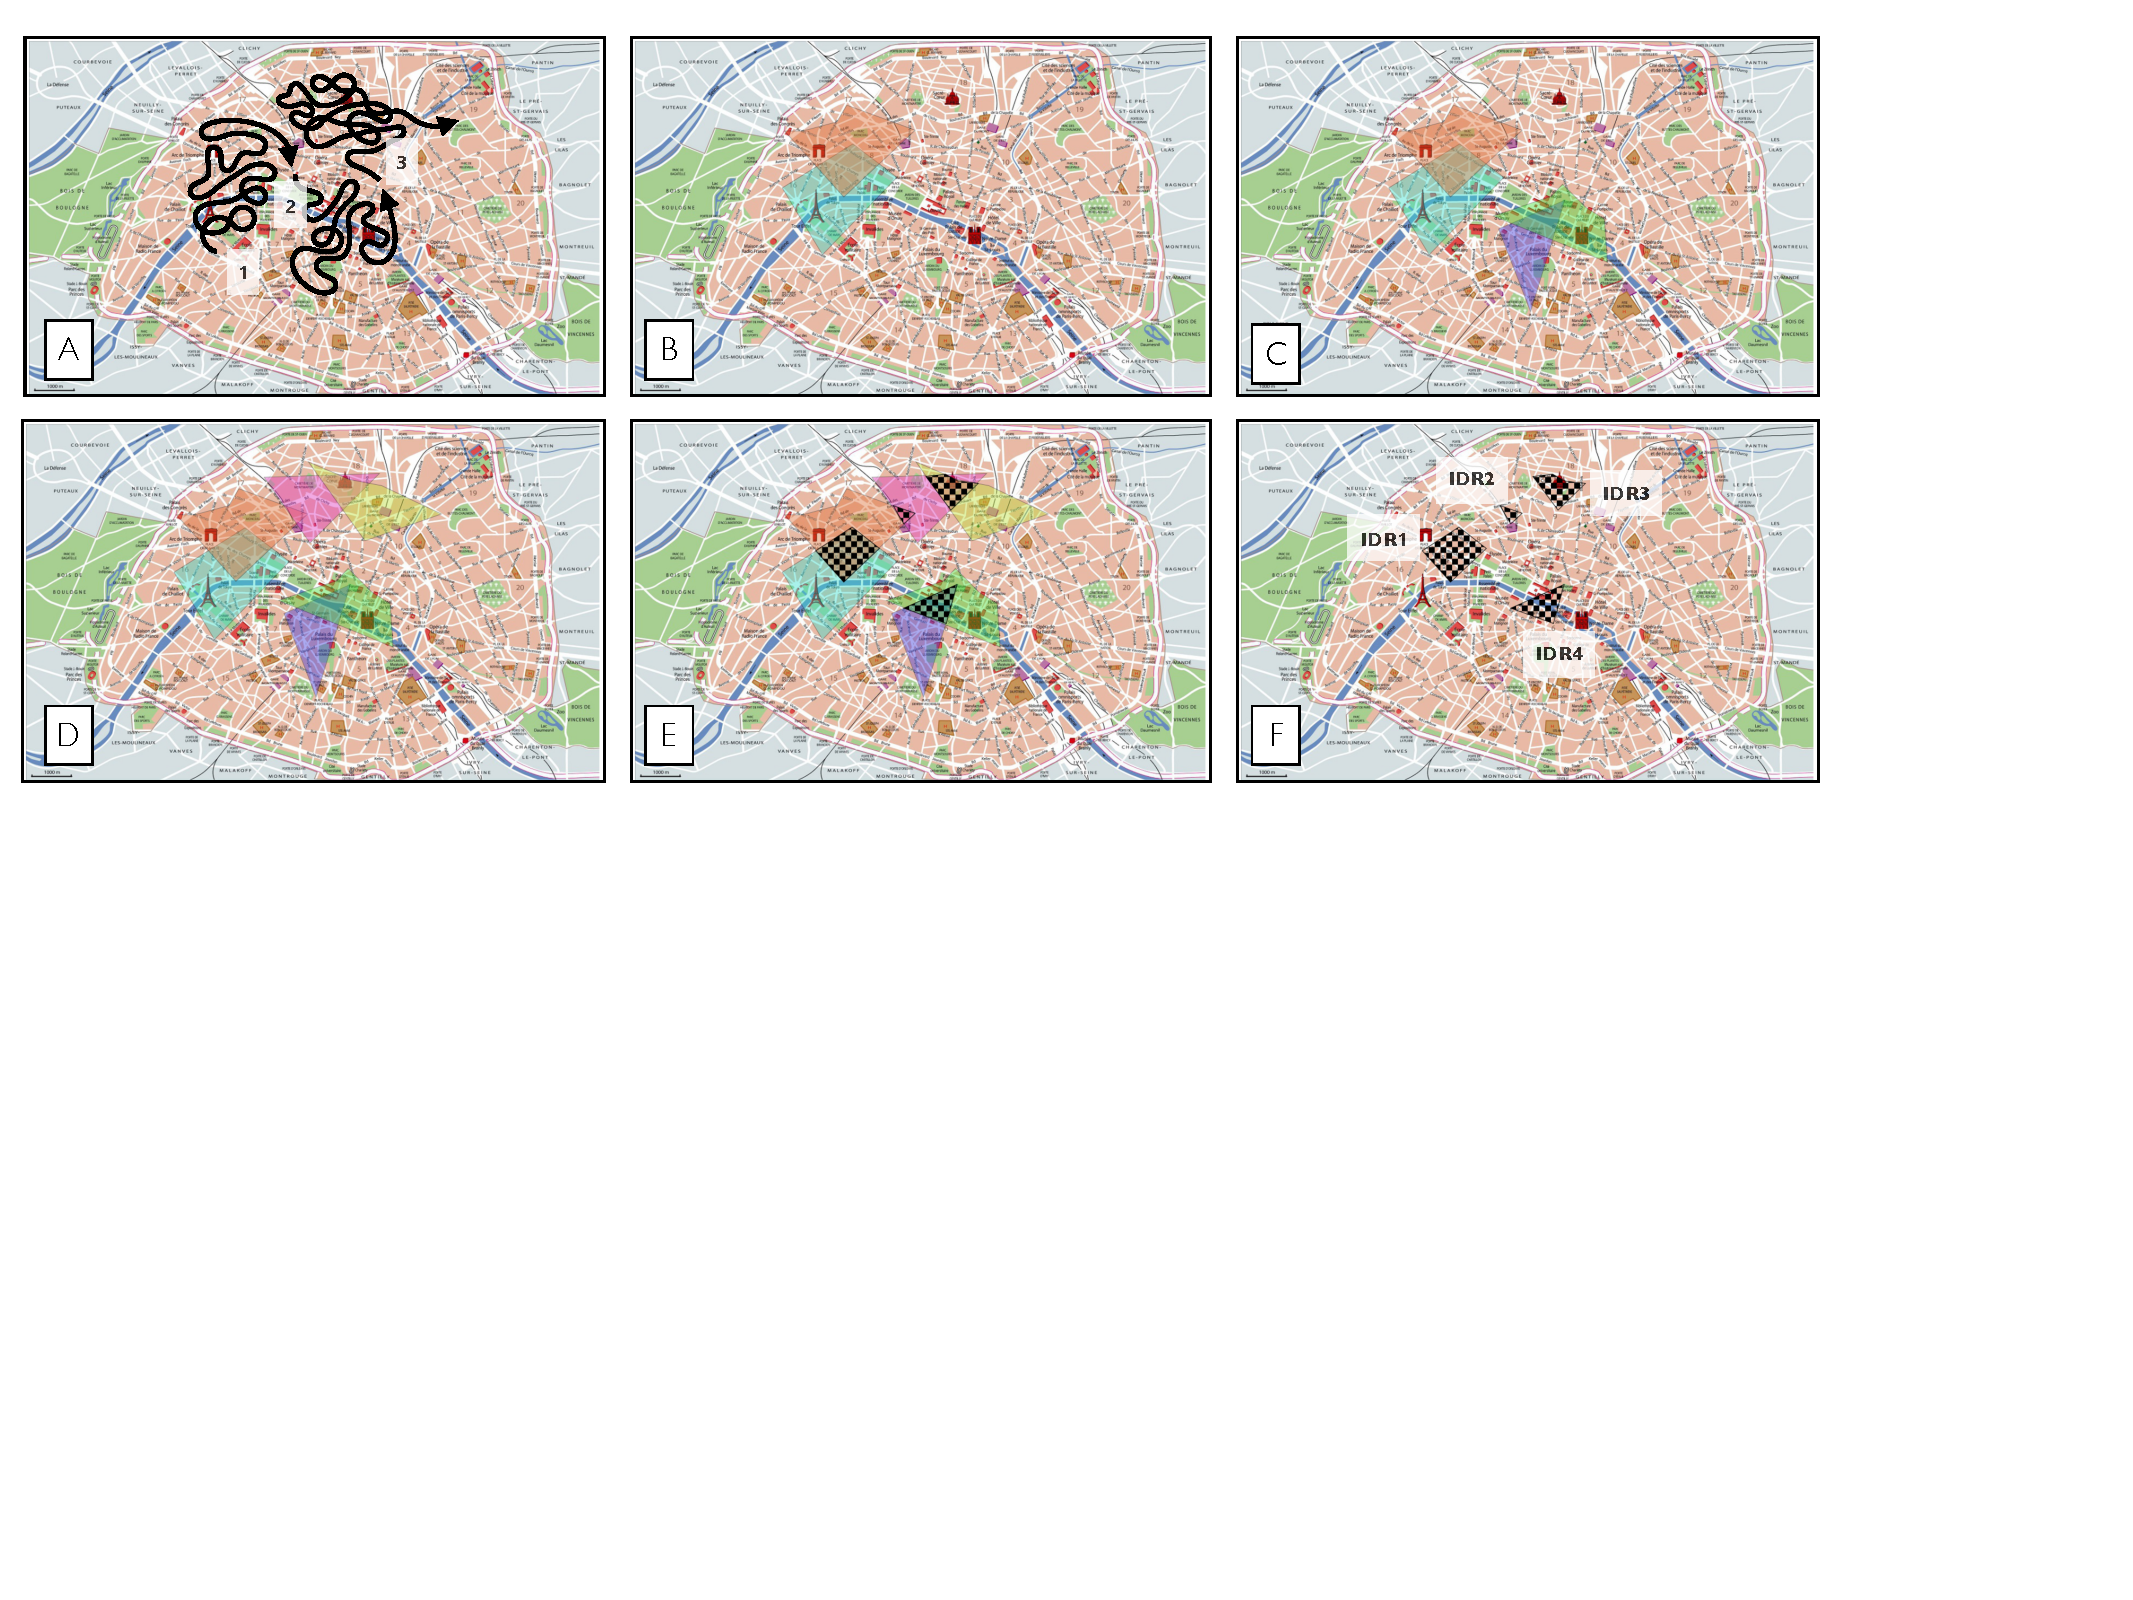
\includegraphics[width=\textwidth]{imagens/regions}
	\caption{O processo de explorar estadias em Paris.}
	\label{fig:regions}
\end{figure}

{\bf Exemplo.} {\em Lucas está planejando passar alguns dias em Paris, França. Sua apreciação pela cultura francesa faz como que ele tenha interesse em novas experiências na cidade. Ele decidiu por alugar uma estadia pelo Airbnb \footnote{\it http://www.airbnb.com}. Ele gosta de descobrir a cidade, portanto ele é aberto a qualquer tipo de estadia em qualquer região com um leve interesse em ficar perto do centro da cidade. O sistema retorna $4000$ opções diferentes. Como ele não tem outras preferências, uma investigação exaustiva para avaliar cada região da cidade independentemente é necessário, o que é quase impossível. Enquanto estava avaliando algumas opções, ele demostrou interesse na região de  ``Champ de Mars'' (próximo à Torre Eiffel), mas ele esqueceu ou não achou necessário clicar num ponto nessa região. Coletando o feedback do seus movimentos com o mouse no mapa de estadias em Paris, nosso sistema consegue rapidamente detectar o interesse dele na região supracitada e apresentar uma quantidade pequena de opções recomendadas para Lucas.}

Seguimos o exemplo acima para descrever como feedback implícito é coletado na prática. Imagem \ref{fig:regions} mostra os passos de Lucas para explorar estadias em Paris. Imagem \ref{fig:regions}.A mostra os movimentos do mouse dele em diferentes intervalos de tempo. Nesse exemplo, consideramos $g = 3$ e coleta o feedback de Lucas em 3 diferentes intervalos de tempo (evoluindo das Imagens \ref{fig:regions}.B até \ref{fig:regions}.D). Isso mostra que Lucas começou sua busca perto da Torre Eiffel e {\em Arc de Triomphe} (Imagem \ref{fig:regions}.B) e gradualmente mostrou também interesse no sul (Imagem \ref{fig:regions}.C) e norte (Imagem \ref{fig:regions}.D). Todas as interseções entre essas regiões são descobertas (regiões tachadas na Imagem \ref{fig:regions}.E), o que representa um conjunto de Regiões de Denso Interesse (IDR, em inglês, {\em Interesting Dense Regions}), isto é IDR1 até IDR4.

E se Lucas quiser voltar para Paris próximo ano? Ele teria que repetir a mesma anális exploratória, a não ser que ele lembre a localização exata das estadias que ele mostrou no ano passado. Usando nosso sistema, ele não precisaria lembrar, porque suas preferências foram coletadas e poderiam ser usadas para realçar um subconjunto similar ao do ano anterior.

No contexto da análise explorátoria, o analista talvez mude suas preferências entre as sessões (por exemplo, no inverno, Lucas talvez queira ficar próximo ao Torre Eiffel, mas no verão, ele talvez não queira). Afim de atacar esse desafio, também implementamos uma análise temporal para identificar padrões em como as preferências do analistas mudam entre as sessões o que permite nosso método de realçamento ser mais preciso e consistente com o interesse do analista.

\section{Objetivos}

Nessa seção, definimos os objetivos gerais e específicos do nosso trabalho.

\subsection{Objetivos Gerais}

\begin{itemize}
	\item Propor uma abordagem de orientação para exploração de dados espaciais considerando o contexto temporal;
	\item Elaborar como análise temporal pode ser efetivamente aplicada na exploração de dados.
\end{itemize}

\subsection{Objetivos Específicos}

\begin{itemize}
	\item Descrever nosso modelo de dados usado para análise temporal;
	\item Descrever nosso conceito de em Região de Denso Interesse usado para captura de feedback;
	\item Apresentar resultados para nossa abordagem;
\end{itemize}

\section{Organização}

Os próximos capítulos estão organizados na seguinte maneira: no Capítulo \ref{chap:contextualizacao} discutimos o estado da arte por trás desse trabalho; Capítulo \ref{chap:modelo} define o modelo de dados; Capítulo \ref{chap:coletando} apresenta como é feito a coleta de feedback durante a análise exploratória; Capítulo \ref{chap:aplicando} demostra como a análise temporal é aplicada; Capítulo \ref{chap:guiando} apresenta como é realizado o realçamento de pontos de interesse do usuário afim de guiá-lo com base no feedback coletado; Capítulo \ref{chap:experimentos} descreve os experimentos e seus resultados; Capítulo \ref{chap:conclusao} conclui e propôe futuros trabalhos.

	\chapter{Contextualização}
\label{chap:contextualizacao}

Este capítulo dá uma visão geral sobre os trabalhos relacionados acerca de exploração de feedback, métodos de destacamento de informações e aplicação de análises temporais. Também é apresentado o sistema que está sendo estendido neste trabalho.

\section{Trabalhos Relacionados}

A literatura na análise de dados espaciais possui um foco na eficiência das iterações exploratórias. A abordagem comum é projetar índices pré-processados, os quais permitem a consulta eficiente de dados espaciais \cite{lins2013nanocubes}. No entanto, também é preciso direcionar a atenção para o {\em valor} dos dados espaciais, porque é muito comum encontrar um analista se perdendo numa enorme quantidade de pontos geográficos. Para solucionar esse problema, ambientes de visualização, como, por exemplo, Tableau\footnote{\it http://www.tableau.com}, Exhibit\footnote{\it http://www.simile-widgets.org/exhibit/}, Spotfire\footnote{\it  http://spotfire.tibco.com}, oferecem funcionalidades para manipular os dados como filtros, consultas agregadores, entre outras. Entretanto essas funcionalidades não se mostram eficazes, visto que nessas ferramentas o pesquisador precisa saber exatamente o que procura. Este trabalho combina a exploração de feedback, métodos de destacamento de informações e análise temporal a fim de otimizar a análise exploratória.

\subsection{Exploração de Feedback}

O modelo espaço-temporal proposto aprimora o processo de análise de dados espaciais destacando subconjuntos de pontos geográficos com base no feedback coletado durante a exploração do analista. Na literatura, há vários trabalhos sobre exploração de feedback para orientar o analista nas futuras iterações da análise como, por exemplo, \citeonline{boley2013one}. A abordagem comum é uma metodologia {\em top-$k$} para reduzir o escopo da consulta baseado no feedback explícito e recomendar um pequeno subconjunto de resultados interessantes de tamanho $k$. Uma clara distinção do presente trabalho é que não busca-se reduzir o escopo, mas alavancar o conjunto de dados com resultados potencialmente interessantes que o analista talvez não tenha notado devido ao enorme volume de dados espaciais. Enquanto as escolhas do analista são limitadas por $k$ em algoritmos de {\em top-$k$} processamento, a abordagem proposta oferece a liberdade de escolha ao mesmo tempo que pontos geográficos vão sendo transparentemente destacados com base nas novas escolhas do analista.

\subsection{Métodos de Destacamento de Informação}

\todo{fala de cada um}

Há trabalhos na literatura sobre métodos de destacamento de informações, por exemplo: \citeonline{Liang2010,Robinson2011,wongsuphasawat2016voyager,willett2007scented}. Entretanto todos esses métodos são {\em objetivos} e não são aplicáveis para o contexto de orientação espacial onde o feedback do usuário é envolvido. Em termos de recomendação, algumas abordagens focam na dimensão espacial \cite{Bao2015,Levandoski:2012} enquanto o contexto e a diversidade do resultado é deixado de lado.

\subsection{Aplicações de Análise Temporal}

Existem várias instâncias na literatura que combinam análise temporal com dados espaciais, como \citeonline{baculo2017,balahadia2017,chidean2018,ghahramani2018,kamath2013,lopestexeira2018,ma2017,mijovic2016,tomoki2010,nara2007,zhan2017,zheng2018}. Essas aplicações de análise temporal são em contextos específicos, os quais não envolvem feedback do usuário, mas representam como análise temporal pode ser perspicaz e proveitosa.

\citeonline{baculo2017} e \citeonline{balahadia2017} fazem uso de dados públicos de Manila, capital das Filipinas, combinando dados espaciais, análise temporal e modelos preditivos e mostrando resultados que podem ser utilizados para preparação de um plano de gestão pública eficaz. \citeonline{ma2017} e \citeonline{zheng2018} também fazem análises realistas de como eventos, como protestos, impactam nas trajetórias de táxis, cujos resultados podem auxiliar no controle de tráfego urbano e nos planos de serviços de transporte da cidade. Ambos realizam ricas análises, as quais contribuíram como inspiração neste trabalho.

\citeonline{chidean2018} apresenta como detectar padrões espaço-temporais no contexto do uso de energia eólica na Península Ibérica usando o algoritmo {\em Second-Order Data-Coupled Clustering}. Apesar do estudo detalhado, esse trabalho não contempla um contexto de análise exploratória.

\citeonline{ghahramani2018}, \citeonline{lopestexeira2018} e \citeonline{zhan2017} demonstram como análise temporal pode ser aplicada no contexto geográfico. \citeonline{zhan2017} vai além gerando uma árvore de clusterização hierárquica. Apesar dos métodos e resultados serem bem detalhados nos trabalhos, essas contribuições não se aplicam ao assunto em questão.

\citeonline{kamath2013} propõe uma abordagem de {\em reinforcement learning} para prever eventos (adoção de {\em memes}) num contexto espaço-temporal. \citeonline{nara2007} introduz um modelo de visualização 3D para dados espaço-temporais que ajuda a analisar qualitativa e quantitativamente os padrões e tendências espaço-temporais. Ambos os trabalhos contribuem para representar como o modelo proposto pode ser combinado com diversas técnicas.

\section{GeoGuide}

\begin{figure}[t]
	\centering
	\includegraphics[width=\columnwidth]{imagens/framework}
	\caption{Componentes do GeoGuide}
	\label{fig:framework}
	\vspace{-10pt}
\end{figure}

\abrv[TADS -- Tecnologia em Análise e Desenvolvimento de Sistemas]{}
\abrv[IFRN -- Instituto Federal do Rio Grande do Norte]{}

GeoGuide \cite{omidvarTehrani2017} é fruto de um projeto de pesquisa realizado por alunos do curso de Tecnologia em Análise e Desenvolvimento de Sistemas (TADS) no Instituto Federal do Rio Grande do Norte (IFRN) em colaboração com a Universidade de Grenoble. Esse projeto se trata de um ambiente de visualização de dados espaciais que coleta as preferências do usuário durante a exploração para destacar subconjuntos de pontos geográficos que podem ser interessantes ao analista. Figura \ref{fig:framework} ilustra os principais componentes da arquitetura do GeoGuide explorados nas próximas subseções.

Neste trabalho, o GeoGuide é potencializado à dois novos conceitos: $i$. regiões densas interessantes e $ii$. análise temporal das preferências do usuário. Esses dois conceitos serão explorados no próximo capítulo.

\subsection{Pré-processamento}

GeoGuide realiza um passo de pré-processamento para criar os índices que serão usados durante a fase de destacamento. O índice é uma tabela comparativa entre todos os pontos usando duas métricas de qualidade: relevância e diversidade. Os valores calculados são normalizados no intervalo de $0.0$ à $1.0$.

\subsubsection{Relevância e Diversidade}

\begin{figure}[t]
	\centering
	\includegraphics[width=\columnwidth]{imagens/exemplo-de-pontos}
	\caption{Exemplo de pontos geográficos com seus atributos}
	\label{fig:exemplo-pontos}
	\vspace{-10pt}
\end{figure}

Relevância representa o quão similar é o ponto $a$ com o ponto $b$ num conjunto de dados. GeoGuide usa a relevância para destacar pontos similares ao feedback do analista. Diversidade representa quão distante o ponto $a$ está localizado do ponto $b$. GeoGuide usa a diversidade para permitir ao analista explorar diferentes regiões, mas ainda assim trabalhar com pontos relevantes ao seu interesse.

\begin{table}[!h]
	\centering
	\begin{tabular}{|c|c|r|r|}
	\hline
	\multicolumn{1}{|c|}{\textbf{Ponto A}} & \multicolumn{1}{c|}{\textbf{Ponto B}} & \multicolumn{1}{c|}{\textbf{Relevância}} & \multicolumn{1}{c|}{\textbf{Diversidade}} \\ \hline
	1                                      & 2                                     & 0.8                                      & 0.9                                       \\ \hline
	1                                      & 3                                     & 0.25                                     & 0.2                                       \\ \hline
	1                                      & 4                                     & 0.9                                      & 0.45                                      \\ \hline
	2                                      & 3                                     & 0.2                                      & 1.0                                       \\ \hline
	2                                      & 4                                     & 1.0                                      & 0.48                                      \\ \hline
	3                                      & 4                                     & 0.2                                      & 0.3                                       \\ \hline
	\end{tabular}
	\caption{Exemplo de Índice de Relevância e Diversidade para pontos na Figura \ref{fig:exemplo-pontos}}
	\label{table:exemplo-indice}
\end{table}

Na Figura \ref{fig:exemplo-pontos}, tem-se, por exemplo, pontos geográficos que representam viagens de táxi. Cada ponto (1, 2, 3 e 4), possui seus atributos: preço da viagem, duração da viagem e a quantidade de passageiros; e sua localização geográfica. Na tabela \ref{table:exemplo-indice}, ilustra-se o exemplo do índice calculado diante dos pontos apresentados na Figura \ref{fig:exemplo-pontos}. Percebe-se que os pontos mais similares entre si são os pontos 2 e 4, enquanto que 2 e 3 são os mais distantes, ou seja, possuem o maior valor de diversidade.


\subsection{Preferências do Usuário}

Para coletar as preferências do usuário, GeoGuide usa ambos feedback implícito e explícito. Feedback explícito é quando o usuário está analisando os atributos de um ponto, por exemplo a descrição de uma casa no Airbnb, e explicitamente pede para explorar pontos similares ao selecionado. Feedback implícito é coletado através da captura dos movimentos do mouse e métricas como  ``quanto tempo o usuário passou analisando o perfil de um ponto''.

\subsection{Destacamento de Dados Espaciais}

GeoGuide combina o índice pré-processado e o feedback coletado para destacar subconjuntos de dados espaciais de acordo com as preferências do analista. O processo de destacamento provou ser eficiente em termos de ``quantos passos o analista leva até completar a tarefa de encontrar um ponto com um determinado perfil''. Usando GeoGuide, analistas foram capazes de completar a tarefa usando, em média, 10.7 passos, enquanto que usando Tableau, foram necessários 43 passos \cite{omidvarTehrani2017}.

% \vspace{25pt}
% \endsubsection

% \closesubsection

	\chapter{Definição do Modelo}
\label{chap:modelo}

Neste capítulo, entendemos as Regiões Densas Interessantes e definimos o modelo espaço-temporal.

\section{Regiões Densas Interessantes}

Uma Região Densa Interessante (IDR, do inglês {\em Interesting Dense Region}) é uma região espacial com uma alta probabilidade de conter pontos de interesse do analista. IDR são coletadas e definidas durante o processamento do feedback do usuário. Diferentemente da literatura que predominantemente foca em intereções explícitos (como clicar no botão, abrir o perfil do ponto), investigamos o feedback implícito.

Durante a exploração iterativa de dados espaciais, é comum o caso que o analista avalia algumas regiões de interesse, mas esquece de dá um feedback explícito sobre aquela região. O ato do usuário olhar para essa região pode ser capturado através do rastreio da movimentos oculares e, como \citeonline{arapakis2014user} mostra, esse método possui uma forte relação com a atenção do usuário.

Entretanto o rastreamento dos movimentos oculares fere várias questões de privacidade, assim sendo optamos pela alternativa de rastrear os deslocamentos do cursor do mouse. \citeonline{arapakis2014understanding} argumenta que esse método possui uma forte relação com o engajamento do usuário. Intuitivamente, um ponto espacial recebe um feedback positivo se o cursor do mouse se desloca próximo a ele frequentemente.

Continua...

\section{Spatial layer}

Each point in a dataset ($p \in \mathcal{P}$) is described using its coordinates (latitude and longitude) and also associated with a set of attributes ($dom(p)$). For instance, TODO

\section{Interesting Dense Regions}

TODO

We have IDRs per iteration/session where implicit feedback is captured such mouse moves (or eye gaze). In the beginning, each IDRs is a group of raw points described using its coordinates (latitude and longitude) and a timestamp (the unix timestamp it was captured). These raw points once captured will enter the clustering (for now, ST-DBSCAN) phase to generate the IDR itself with a profile. The profile is built based on the spatial layer and it should represent a summary of its contained points from the spatial layer.

\begin{itemize}
	\item A profile has summary of its spatial points number attributes. For each number attribute in $dom(p)$, we calculate the average, median and standard deviation based on the points contained in the IDR.

	\item A profile has a word rank $R$ of the terms in the text attributes of its spatial points. For each text attribute in $dom(p)$, we evaluate the most used terms in order to create a word rank \cite{kumar2017}.

	\item A profile has a map $M$ between the $<name, value>$ of categoricals attributes and its relevance in $dom(p)$.

	\item TODO: datetime attributes

	\item A profile has a meta property with values such the count of points in the IDR.
\end{itemize}

\section{Highlighting}

TODO
	\chapter{Considerações Finais}
\label{chap:conclusao}

Neste trabalho é proposto um modelo de análise espaço-temporal para identificação de padrões nas preferências coletadas pela ferramenta GeoGuide enquanto um analista realiza a análise exploratória de dados espaciais. O modelo proposto mostra-se eficiente para ser utilizado a fim de aprimorar o uso da captura de feedback implícito para orientar o usuário nas próximas iterações através do método de destacamento de pontos geográficos.

\section{Contribuições}

O modelo propõe 2 novos conceitos: $i$. regiões densas interessantes e $ii$. análise temporal das preferências do usuário. As regiões densas interessantes (IDR) representam as preferências do analista no contexto espacial no determinado momento. Cada IDR possui também um perfil que representa as preferências do analista no contexto de domínio.

As regiões e seus perfis permitem a análise temporal das preferências do usuário. Os métodos para análise em ambos contextos espaciais e de domínio são investigados e apresentados com o propósito de identificar padrões nas iterações da análise exploratória.

\section{Trabalhos futuros}

Os dados gerados pelo modelo proposto podem futuramente ser explorados em diversos cenários. Por exemplo, os dados gerados podem ser utilizados para entender as preferências de um grupo de analistas a fim de potencializar o descobrimento de objetivos comuns entre eles.

No que diz respeito aos ambientes de exploração de dados espaciais, os dados coletados podem ser combinados com algoritmos preditivos para responder questionamentos como ``onde o analista deve está interessado na próxima iteração?'' ou até mesmo ``será que o analista está interessado nesse apartamento com varanda?''.  

  \backmatter

  % Bibliografia (arquivo Capitulos/Referencias.bib)
  %\nocite{*}
  \postextual
  \bibliography{capitulos/referencias}
  %\bibliographystyle{abnt-alf}

  % Apêndice A (arquivo Includes/ApendiceA)
%   \begin{apendicesenv}
%     %\partapendices

%     \include{capitulos/ApendiceA}
%   \end{apendicesenv}

  % Anexo A (arquivo Includes/AnexoA)
%   \begin{anexosenv}
%     \partanexos
%     \include{capitulos/AnexoA}
%   \end{anexosenv}

\phantompart
\printindex

\end{document}


% % Hifeniza������o de palavras feita de forma incorreta pelo LaTeX
% \hyphenation{PYTHON ou-tros}


% % Inicio do documento
% \begin{document}

% \frenchspacing

% % Capa (arquivo Includes/Capa.tex)
% % Capa
% Prote��o externa do trabalho e sobre a qual se imprimem as informa��es indispens�veis 
% � sua identifica��o.

% Especifica��o da capa
\begin{titlepage}
	\begin{center}
		
		  
		\begin{minipage}{11.15cm}
			\begin{center}
				\begin{espacosimples}
					{\small \ \\
                       \textsc{Instituto Federal do Rio Grande do Norte}
                       \\
							  \textsc{Campus Natal - Central}					\\
							  \textsc{Diretoria de Gestão e Tecnologia da Informação}	   
							  \\
							  \textsc{Tecnologia em Análise e Desenvolvimento de Sistemas}}   	
                       \\
				\end{espacosimples}
			\end{center}
		\end{minipage}

			
		\vspace{6cm}
						
		% T�tulo do trabalho
		{\setlength{\baselineskip}%
		{1.3\baselineskip}
		{\LARGE \textbf{Título do trabalho}}\par}
			
		\vspace{3cm}
			
		% Nome do aluno (autor)
		{\large \textbf{Nome completo do autor}}
						
		\vspace{6cm}
		
		% Local da institui��o onde o trabalho deve ser apresentado e ano de entrega do mesmo
		Natal-RN\\Mês (por extenso) e ano
	\end{center}
\end{titlepage}

% % Folha de rosto (arquivo extra-includes/FolhaRosto.tex)
% % Folha de rosto
% Cont�m os elementos essenciais � identificação do trabalho.

% T�tulo, nome do aluno e respectivo orientador e filiação
\titulo{\Large{Implementação e Análise de Algoritmos para Solução do Cubo de Rubik}}
\autor{Camila Jordana Ribeiro Teixeira}
\orientador[Orientador]{\par Prof. Dr. Plácido Antônio de Souza Neto}
\instituicao
{
   TADS -- Curso de Tecnologia em Análise e Desenvolvimento de
   Sistemas\par 
   DIATINF -- Diretoria Acadêmica de gestão e Tecnologia da Informação\par 
   CNAT -- Campus Natal - Central\par 
   IFRN -- Instituto Federal do Rio Grande do Norte }
	
% Natureza do trabalho (não deve ser modificada)
\comentario
{
	Trabalho de conclusão de curso de graduação do curso de Tecnologia em Análise e
	Desenvolvimento de Sistemas da Diretoria de Gestão e Tecnologia de Informação
	do Instituto Federal do Rio Grande do Norte como requisito parcial para a
	obtenção do grau de Tecnólogo em Análise e Desenvolvimento de
	Sistemas.\bigskip\\
   \textit{Linha de pesquisa}:\\Análise de Algoritmos
}
		
% Local e data
\local{Natal-RN}
\data{Dezembro - 2017}
	
\folhaderosto

% % Folha de aprovacao (arquivo extra-includes/FolhaAprovacao.tex)
% % Folha de aprova��o
\begin{folhadeaprovacao}
	\setlength{\ABNTsignthickness}{0.4pt}
	\setlength{\ABNTsignwidth}{10cm}
	
	\noindent 
	Trabalho de Conclusão de Curso de Graduação sob o título
	\textit{Título} apresentada por Nome completo do autor e aceita pelo Diretoria
	de Gestão e Tecnologia da Informação do Instituto Federal do Rio Grande do
	Norte, sendo aprovada por todos os membros da banca examinadora abaixo especificada:
		
	% Membros da banca examinadora e respectivas filia��es
	\assinatura
	{
		Nome completo do orientador e titulação   			                  \\
		{\small Presidente}											          \smallskip\\ 
		{\footnotesize
			DIATINF -- Diretoria Acadêmica de Gestão e Tecnologia da Informação		   \\
		  	IFRN -- Instituto Federal do Rio Grande do Norte
		}
   }
      
   \assinatura
	{
      Nome completo do examinador e titulação   			                  \\
		{\small Examinador}											          \smallskip\\ 
		{\footnotesize
			Diretoria/Departamento		\\
		  	Instituto
		}
   }   
   
   \assinatura
	{
      Nome completo do examinador e titulação   			                  \\
		{\small Examinador}											          \smallskip\\ 
		{\footnotesize
			Diretoria/Departamento		\\
		  	Universidade
		}
	}
		
	\vfill
	
	\begin{center}
		Natal-RN, data da defesa (dia, mês e ano).
	\end{center}
\end{folhadeaprovacao}


% % Dedicatoria (arquivo extra-includes/Dedicatoria.tex)
% % Dedicat�ria


% \vspace{15cm}
% \begin{flushright}
	
% \end{flushright}


\begin{dedicatoria}
	\vspace*{\fill}
	\begin{flushright}
		Aos meus pais que nunca duvidaram de mim.
	\end{flushright}
	\vspace{4cm}
\end{dedicatoria}

% % Agradecimentos (arquivo extra-includes/Agradecimentos.tex)
% % Agradecimentos

\chapter*{Agradecimentos}

Ao meu orientador \mySupervisorName, pelo seu empenho em sempre buscar extrair o melhor de mim.

À Behrooz Omidvar-Tehrani, pelas suas colaborações mesmo estando a um oceano de distância.

À Francisco Bento da Silva Júnior, pelas suas contribuições como amigo e colega de pesquisa.

% % Epigrafe (arquivo extra-includes/Epigrafe.tex)
% % Ep�grafe (cita��o seguida de indica��o de autoria)

\chapter*{}
\vspace{15cm}
\begin{flushright}
	\textit
	{
		Se você for curioso, encontrará quebra-cabeças em torno de você. Se você estiver determinado, irá resolvê-los.
	}\medskip\\ 
	Erno Rubik
\end{flushright}

% % Resumo em l���ngua vernacula (arquivo extra-includes/Resumo.tex)
% % Resumo
\begin{center}
	{\Large{\textbf{\myThesis}}}
\end{center}

\vspace{1cm}

\begin{flushright}
	Autor: \myName\\
	Orientador(a): \mySupervisorName
\end{flushright}

\vspace{1cm}

\begin{center}
	\Large{\textsc{\textbf{Resumo}}}
\end{center}

\noindent O resumo deve apresentar de forma concisa os pontos relevantes de um
texto, fornecendo uma visão rápida e clara do conteúdo e das conclusões do
trabalho. O texto, redigido na forma impessoal do verbo, é constituído de uma
sequência de frases concisas e objetivas e não de uma simples enumeração de
tópicos, não ultrapassando 500 palavras, seguido, logo abaixo, das palavras
representativas do conteúdo do trabalho, isto é, palavras-chave e/ou
descritores. Por fim, deve-se evitar, na redação do resumo, o uso de parágrafos
(em geral resumos são escritos em parágrafo único), bem como de fórmulas,
diagramas e símbolos, optando-se, quando necessário, pela transcrição na forma
extensa, além de não incluir citações bibliográficas.

\noindent\textit{Palavras-chave}: Palavra-chave 1, Palavra-chave 2, Palavra-chave 3.

% % Abstract, resumo em l���ngua estrangeira (arquivo Include/Abstract.tex)
% % Resumo em l�ngua estrangeira (em ingl�s Abstract, em espanhol Resumen, em franc�s R�sum�)
\begin{center}
	{\Large{\textbf{Sentiment analysis model to extract data from social network}}}
\end{center}

\vspace{1cm}

\begin{flushright}
	Author: Yuri Jordan de Melo Oliveira\\
	Supervisor: Prof. Plácido Antônio de Souza Neto, Ph.D.
\end{flushright}

\vspace{1cm}

\begin{center}
	\Large{\textsc{\textbf{Abstract}}}
\end{center}

\noindent Is noticed that, currently, the technical ability to collect, analyse and use information about humans`s opinions and thoughts, has its development boosted because of the spread of the social networks, to a world scale, these capabilities, have been applied for the understanding and decision-making, in the various areas of society such as health, education, politics and economy. An exploratory is made and a model for the analysis of textual data extracted from social networks is developed, in order to know if, what the users of these networks write in them, has a positive, neutral or negative feeling. To achieve this, it is necessary to generate a model for this type of analysis, implement the necessary algorithms for this purpose and a web service, in order to expose these algorithms and applying them in a case study, with some of the pre-candidates for the presidency of the Republic of Brazil, in 2018. It is then done, an exploratory research about. Therefore, 2470 messages were collected and analyzed, being classified as negative, neutral or positive and marked on a map, the place from which they came.

\noindent Keywords:  Sentiment analysis, Natural Language Processing, Social network.





% % Lista de figuras
% \listoffigures

% % Lista de tabelas
% \listoftables

% % Lista de abreviaturas e siglas
% \listadeabreviaturas

% % Lista de símbolos
% % \listadesimbolos

% % Lista de algoritmos (se houver)
% % Devem ser inclu���dos os pacotes algorithm e algorithmic
% \listofalgorithms

% % Sum���rio
% \sumario

% % Parte central do trabalho, englobando os cap��tulos que constituem o mesmo
% % Os referidos cap��tulos devem ser organizados dentro do diret��rio "Cap��tulos"

% % Capitulo 1: Introdu����o (arquivo Includes/Introducao.tex)
% \chapter{Introdução}
\label{chap:introducao}

Mais do que nunca estamos sobrecarregados com a quantidade de dados que criamos a cada dia. Quando comparamos quanto de informação vem sendo gerada nos ultimos anos, percebemos que está aumentando significamente. Além dessa evolução quantitativa, hoje temos os mais diversos tipos de informação, por exemplo: documentos, tuítes, fotos, vídeos, \textit{GIFs}, \textit{check-ins} entre vários outros.

Esse fenômeno vem sido chamado de \textit{Big Data} e representa uma crescente área de estudo atualmente. Como consequência, pesquisadores estão analisando e aprendendo com essas informações geradas, entretanto o crescimento contínuo da quantidade de dados dificulta as análises. Portanto pessoas estão investindo em novas técnicas e ferramentas para romper desafios como mineração de dados, {\em data cleaning}, visualização de dados, classificação de dados, exploração de dados e muito mais.

Um tipo comum de dados é o que chamamos de dado espacial, o qual a informação possui atributos geográficos como latitude e longitudade (por exemplo: tuítes, avaliação de restaurantes, {\em check-ins} em estabelecimentos). Dados espaciais podem ser muito significativo, por exemplo, um {\em check-in} no aeroporto por sua irmã na manhã do seu aniversário, provavelmente significa que você terá uma surpresa.

Cada registro em dados espaciais representa uma atividade numa precisa localização geográfica, em outras palavras, a análise desse tipo de dado permite realizar descobertas baseadas em fatos. Analistas estão frequetemente interessados em observar padrões espaciais e tendências para melhorar seus processos de tomada de decisão. Análise de dados espaciais tem várias aplicações como gerenciamento de cidade inteligentes, gerenciamento de disastres e transporte autônomo \cite{RoddickEHPS04,Telang:2012}.

\section{Problema}

A análise de dados espaciais geralmente é realizada num contexto exploratório: o analista não tem uma consulta precisa em mente e ele explora os dados em passos iterativos a fim de encontrar resultados potencialmente interessantes. Tradicionalmente, um cenário de análise exploratória é descrito na seguinte maneira: o analista visualiza um subconjunto de dados usando uma consulta em ambiente de visualização (por exemplo: Tableau\footnote{\it http://www.tableau.com},
Exhibit\footnote{\it http://www.simile-widgets.org/exhibit/},
Spotfire\footnote{\it http://spotfire.tibco.com}); o resultado será ilustrado em um mapa geográfico; então o analista investiga diferentes partes do conjuto de dados movendo ou focando o mapa afim de encontrar padrões ou tendências de interesse. O analista pode iterar por esse processo várias vezes realizando consultas diferentes e focando em diferentes aspectos.

Contudo, a vasto tamanho do conjunto de dados espacias faz com que o analista se sinta perdido durante a exploração. É possível ter milhares de pontos geográficos em cada bairro de uma cidade, por exemplo. Analistas precisam ter acesso apenas a algumas opções (chamadas de ``highlights'') que ajam como uma direção e assim permitir que ele foque no que lhe interessa na análise. No cenário perfeito, essas opções não são aleatoriamente escolhidas e representam o que o analista se mostrou interessado em iterações passadas.

Neste trabalho, formulamos uma solução para ``realçamento de dados usando feedback coletado ao longo do tempo''. Em outras palavras, buscamos realçar alguns pontos geográficos baseado nos interesses do analista afim de guiá-lo na direção ao que ele deve se concentrar nas iterações seguintes do processo de análise.

\subsection{Caso de Estudo}

Nessa seção, vamos apresentar um caso de estudo afim de demostrar a funcionalidade da nossa abordagem na prática.

\begin{figure}[t]
	\centering
	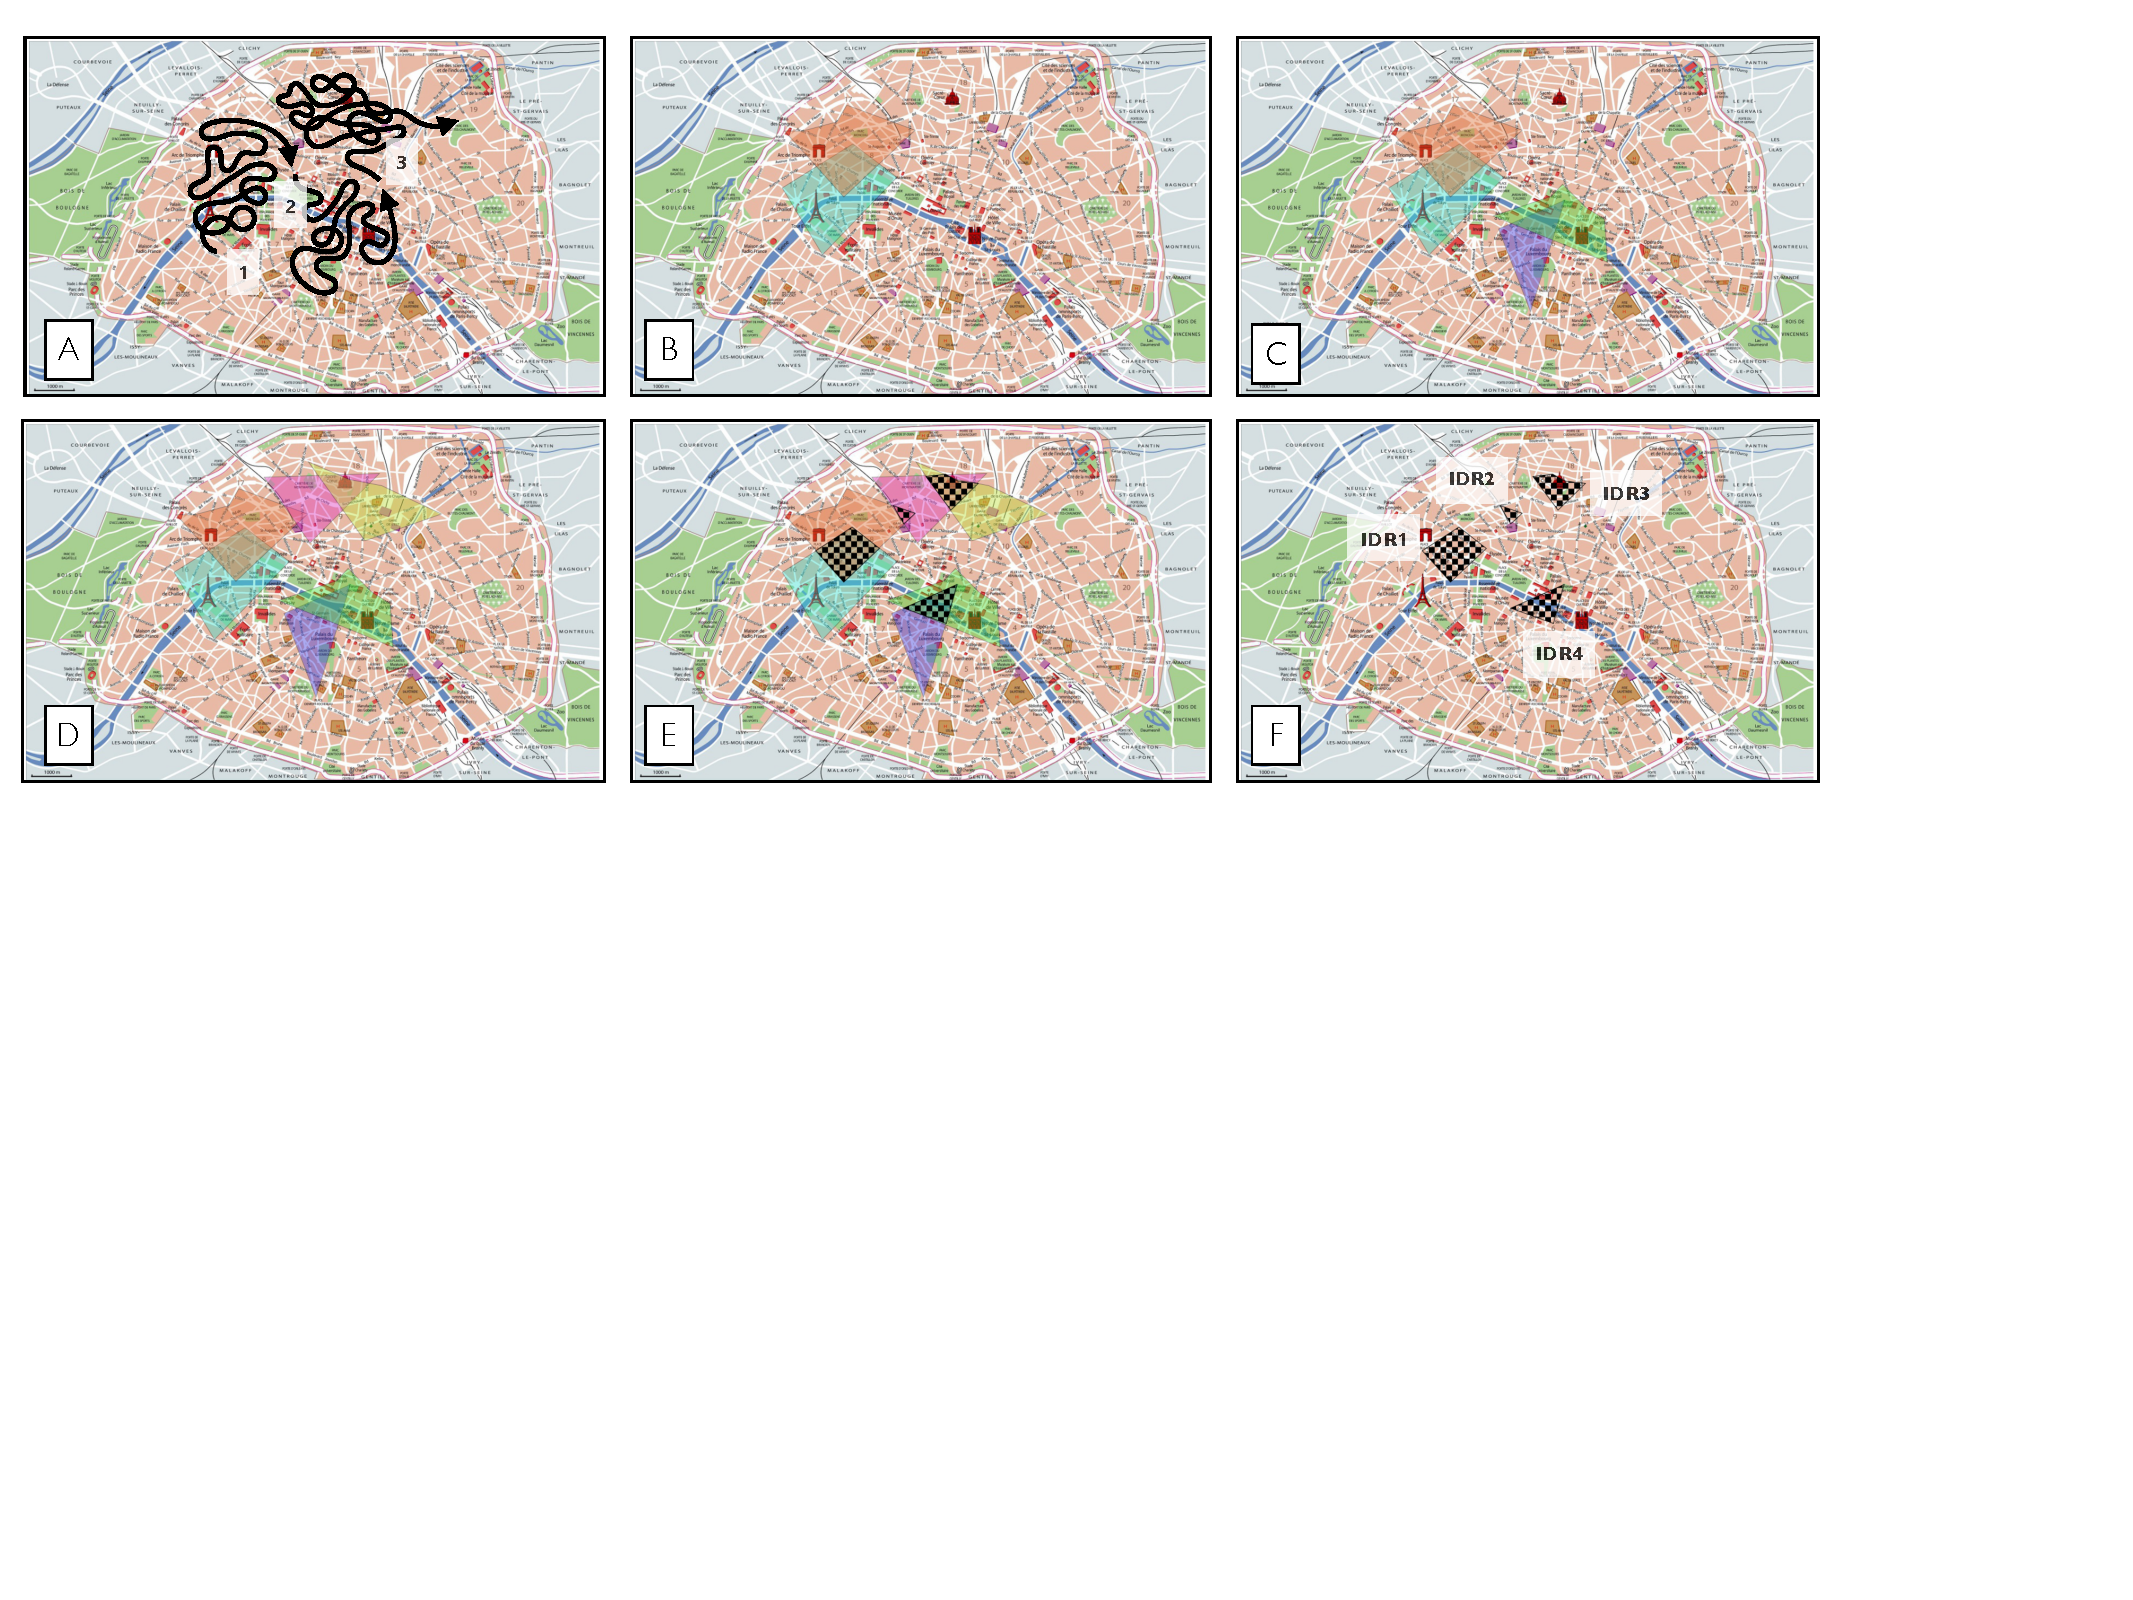
\includegraphics[width=\textwidth]{imagens/regions}
	\caption{O processo de explorar estadias em Paris.}
	\label{fig:regions}
\end{figure}

{\bf Exemplo.} {\em Lucas está planejando passar alguns dias em Paris, França. Sua apreciação pela cultura francesa faz como que ele tenha interesse em novas experiências na cidade. Ele decidiu por alugar uma estadia pelo Airbnb \footnote{\it http://www.airbnb.com}. Ele gosta de descobrir a cidade, portanto ele é aberto a qualquer tipo de estadia em qualquer região com um leve interesse em ficar perto do centro da cidade. O sistema retorna $4000$ opções diferentes. Como ele não tem outras preferências, uma investigação exaustiva para avaliar cada região da cidade independentemente é necessário, o que é quase impossível. Enquanto estava avaliando algumas opções, ele demostrou interesse na região de  ``Champ de Mars'' (próximo à Torre Eiffel), mas ele esqueceu ou não achou necessário clicar num ponto nessa região. Coletando o feedback do seus movimentos com o mouse no mapa de estadias em Paris, nosso sistema consegue rapidamente detectar o interesse dele na região supracitada e apresentar uma quantidade pequena de opções recomendadas para Lucas.}

Seguimos o exemplo acima para descrever como feedback implícito é coletado na prática. Imagem \ref{fig:regions} mostra os passos de Lucas para explorar estadias em Paris. Imagem \ref{fig:regions}.A mostra os movimentos do mouse dele em diferentes intervalos de tempo. Nesse exemplo, consideramos $g = 3$ e coleta o feedback de Lucas em 3 diferentes intervalos de tempo (evoluindo das Imagens \ref{fig:regions}.B até \ref{fig:regions}.D). Isso mostra que Lucas começou sua busca perto da Torre Eiffel e {\em Arc de Triomphe} (Imagem \ref{fig:regions}.B) e gradualmente mostrou também interesse no sul (Imagem \ref{fig:regions}.C) e norte (Imagem \ref{fig:regions}.D). Todas as interseções entre essas regiões são descobertas (regiões tachadas na Imagem \ref{fig:regions}.E), o que representa um conjunto de Regiões de Denso Interesse (IDR, em inglês, {\em Interesting Dense Regions}), isto é IDR1 até IDR4.

E se Lucas quiser voltar para Paris próximo ano? Ele teria que repetir a mesma anális exploratória, a não ser que ele lembre a localização exata das estadias que ele mostrou no ano passado. Usando nosso sistema, ele não precisaria lembrar, porque suas preferências foram coletadas e poderiam ser usadas para realçar um subconjunto similar ao do ano anterior.

No contexto da análise explorátoria, o analista talvez mude suas preferências entre as sessões (por exemplo, no inverno, Lucas talvez queira ficar próximo ao Torre Eiffel, mas no verão, ele talvez não queira). Afim de atacar esse desafio, também implementamos uma análise temporal para identificar padrões em como as preferências do analistas mudam entre as sessões o que permite nosso método de realçamento ser mais preciso e consistente com o interesse do analista.

\section{Objetivos}

Nessa seção, definimos os objetivos gerais e específicos do nosso trabalho.

\subsection{Objetivos Gerais}

\begin{itemize}
	\item Propor uma abordagem de orientação para exploração de dados espaciais considerando o contexto temporal;
	\item Elaborar como análise temporal pode ser efetivamente aplicada na exploração de dados.
\end{itemize}

\subsection{Objetivos Específicos}

\begin{itemize}
	\item Descrever nosso modelo de dados usado para análise temporal;
	\item Descrever nosso conceito de em Região de Denso Interesse usado para captura de feedback;
	\item Apresentar resultados para nossa abordagem;
\end{itemize}

\section{Organização}

Os próximos capítulos estão organizados na seguinte maneira: no Capítulo \ref{chap:contextualizacao} discutimos o estado da arte por trás desse trabalho; Capítulo \ref{chap:modelo} define o modelo de dados; Capítulo \ref{chap:coletando} apresenta como é feito a coleta de feedback durante a análise exploratória; Capítulo \ref{chap:aplicando} demostra como a análise temporal é aplicada; Capítulo \ref{chap:guiando} apresenta como é realizado o realçamento de pontos de interesse do usuário afim de guiá-lo com base no feedback coletado; Capítulo \ref{chap:experimentos} descreve os experimentos e seus resultados; Capítulo \ref{chap:conclusao} conclui e propôe futuros trabalhos.


% \chapter{Contextualização}
\label{chap:contextualizacao}

Este capítulo dá uma visão geral sobre os trabalhos relacionados acerca de exploração de feedback, métodos de destacamento de informações e aplicação de análises temporais. Também é apresentado o sistema que está sendo estendido neste trabalho.

\section{Trabalhos Relacionados}

A literatura na análise de dados espaciais possui um foco na eficiência das iterações exploratórias. A abordagem comum é projetar índices pré-processados, os quais permitem a consulta eficiente de dados espaciais \cite{lins2013nanocubes}. No entanto, também é preciso direcionar a atenção para o {\em valor} dos dados espaciais, porque é muito comum encontrar um analista se perdendo numa enorme quantidade de pontos geográficos. Para solucionar esse problema, ambientes de visualização, como, por exemplo, Tableau\footnote{\it http://www.tableau.com}, Exhibit\footnote{\it http://www.simile-widgets.org/exhibit/}, Spotfire\footnote{\it  http://spotfire.tibco.com}, oferecem funcionalidades para manipular os dados como filtros, consultas agregadores, entre outras. Entretanto essas funcionalidades não se mostram eficazes, visto que nessas ferramentas o pesquisador precisa saber exatamente o que procura. Este trabalho combina a exploração de feedback, métodos de destacamento de informações e análise temporal a fim de otimizar a análise exploratória.

\subsection{Exploração de Feedback}

O modelo espaço-temporal proposto aprimora o processo de análise de dados espaciais destacando subconjuntos de pontos geográficos com base no feedback coletado durante a exploração do analista. Na literatura, há vários trabalhos sobre exploração de feedback para orientar o analista nas futuras iterações da análise como, por exemplo, \citeonline{boley2013one}. A abordagem comum é uma metodologia {\em top-$k$} para reduzir o escopo da consulta baseado no feedback explícito e recomendar um pequeno subconjunto de resultados interessantes de tamanho $k$. Uma clara distinção do presente trabalho é que não busca-se reduzir o escopo, mas alavancar o conjunto de dados com resultados potencialmente interessantes que o analista talvez não tenha notado devido ao enorme volume de dados espaciais. Enquanto as escolhas do analista são limitadas por $k$ em algoritmos de {\em top-$k$} processamento, a abordagem proposta oferece a liberdade de escolha ao mesmo tempo que pontos geográficos vão sendo transparentemente destacados com base nas novas escolhas do analista.

\subsection{Métodos de Destacamento de Informação}

\todo{fala de cada um}

Há trabalhos na literatura sobre métodos de destacamento de informações, por exemplo: \citeonline{Liang2010,Robinson2011,wongsuphasawat2016voyager,willett2007scented}. Entretanto todos esses métodos são {\em objetivos} e não são aplicáveis para o contexto de orientação espacial onde o feedback do usuário é envolvido. Em termos de recomendação, algumas abordagens focam na dimensão espacial \cite{Bao2015,Levandoski:2012} enquanto o contexto e a diversidade do resultado é deixado de lado.

\subsection{Aplicações de Análise Temporal}

Existem várias instâncias na literatura que combinam análise temporal com dados espaciais, como \citeonline{baculo2017,balahadia2017,chidean2018,ghahramani2018,kamath2013,lopestexeira2018,ma2017,mijovic2016,tomoki2010,nara2007,zhan2017,zheng2018}. Essas aplicações de análise temporal são em contextos específicos, os quais não envolvem feedback do usuário, mas representam como análise temporal pode ser perspicaz e proveitosa.

\citeonline{baculo2017} e \citeonline{balahadia2017} fazem uso de dados públicos de Manila, capital das Filipinas, combinando dados espaciais, análise temporal e modelos preditivos e mostrando resultados que podem ser utilizados para preparação de um plano de gestão pública eficaz. \citeonline{ma2017} e \citeonline{zheng2018} também fazem análises realistas de como eventos, como protestos, impactam nas trajetórias de táxis, cujos resultados podem auxiliar no controle de tráfego urbano e nos planos de serviços de transporte da cidade. Ambos realizam ricas análises, as quais contribuíram como inspiração neste trabalho.

\citeonline{chidean2018} apresenta como detectar padrões espaço-temporais no contexto do uso de energia eólica na Península Ibérica usando o algoritmo {\em Second-Order Data-Coupled Clustering}. Apesar do estudo detalhado, esse trabalho não contempla um contexto de análise exploratória.

\citeonline{ghahramani2018}, \citeonline{lopestexeira2018} e \citeonline{zhan2017} demonstram como análise temporal pode ser aplicada no contexto geográfico. \citeonline{zhan2017} vai além gerando uma árvore de clusterização hierárquica. Apesar dos métodos e resultados serem bem detalhados nos trabalhos, essas contribuições não se aplicam ao assunto em questão.

\citeonline{kamath2013} propõe uma abordagem de {\em reinforcement learning} para prever eventos (adoção de {\em memes}) num contexto espaço-temporal. \citeonline{nara2007} introduz um modelo de visualização 3D para dados espaço-temporais que ajuda a analisar qualitativa e quantitativamente os padrões e tendências espaço-temporais. Ambos os trabalhos contribuem para representar como o modelo proposto pode ser combinado com diversas técnicas.

\section{GeoGuide}

\begin{figure}[t]
	\centering
	\includegraphics[width=\columnwidth]{imagens/framework}
	\caption{Componentes do GeoGuide}
	\label{fig:framework}
	\vspace{-10pt}
\end{figure}

\abrv[TADS -- Tecnologia em Análise e Desenvolvimento de Sistemas]{}
\abrv[IFRN -- Instituto Federal do Rio Grande do Norte]{}

GeoGuide \cite{omidvarTehrani2017} é fruto de um projeto de pesquisa realizado por alunos do curso de Tecnologia em Análise e Desenvolvimento de Sistemas (TADS) no Instituto Federal do Rio Grande do Norte (IFRN) em colaboração com a Universidade de Grenoble. Esse projeto se trata de um ambiente de visualização de dados espaciais que coleta as preferências do usuário durante a exploração para destacar subconjuntos de pontos geográficos que podem ser interessantes ao analista. Figura \ref{fig:framework} ilustra os principais componentes da arquitetura do GeoGuide explorados nas próximas subseções.

Neste trabalho, o GeoGuide é potencializado à dois novos conceitos: $i$. regiões densas interessantes e $ii$. análise temporal das preferências do usuário. Esses dois conceitos serão explorados no próximo capítulo.

\subsection{Pré-processamento}

GeoGuide realiza um passo de pré-processamento para criar os índices que serão usados durante a fase de destacamento. O índice é uma tabela comparativa entre todos os pontos usando duas métricas de qualidade: relevância e diversidade. Os valores calculados são normalizados no intervalo de $0.0$ à $1.0$.

\subsubsection{Relevância e Diversidade}

\begin{figure}[t]
	\centering
	\includegraphics[width=\columnwidth]{imagens/exemplo-de-pontos}
	\caption{Exemplo de pontos geográficos com seus atributos}
	\label{fig:exemplo-pontos}
	\vspace{-10pt}
\end{figure}

Relevância representa o quão similar é o ponto $a$ com o ponto $b$ num conjunto de dados. GeoGuide usa a relevância para destacar pontos similares ao feedback do analista. Diversidade representa quão distante o ponto $a$ está localizado do ponto $b$. GeoGuide usa a diversidade para permitir ao analista explorar diferentes regiões, mas ainda assim trabalhar com pontos relevantes ao seu interesse.

\begin{table}[!h]
	\centering
	\begin{tabular}{|c|c|r|r|}
	\hline
	\multicolumn{1}{|c|}{\textbf{Ponto A}} & \multicolumn{1}{c|}{\textbf{Ponto B}} & \multicolumn{1}{c|}{\textbf{Relevância}} & \multicolumn{1}{c|}{\textbf{Diversidade}} \\ \hline
	1                                      & 2                                     & 0.8                                      & 0.9                                       \\ \hline
	1                                      & 3                                     & 0.25                                     & 0.2                                       \\ \hline
	1                                      & 4                                     & 0.9                                      & 0.45                                      \\ \hline
	2                                      & 3                                     & 0.2                                      & 1.0                                       \\ \hline
	2                                      & 4                                     & 1.0                                      & 0.48                                      \\ \hline
	3                                      & 4                                     & 0.2                                      & 0.3                                       \\ \hline
	\end{tabular}
	\caption{Exemplo de Índice de Relevância e Diversidade para pontos na Figura \ref{fig:exemplo-pontos}}
	\label{table:exemplo-indice}
\end{table}

Na Figura \ref{fig:exemplo-pontos}, tem-se, por exemplo, pontos geográficos que representam viagens de táxi. Cada ponto (1, 2, 3 e 4), possui seus atributos: preço da viagem, duração da viagem e a quantidade de passageiros; e sua localização geográfica. Na tabela \ref{table:exemplo-indice}, ilustra-se o exemplo do índice calculado diante dos pontos apresentados na Figura \ref{fig:exemplo-pontos}. Percebe-se que os pontos mais similares entre si são os pontos 2 e 4, enquanto que 2 e 3 são os mais distantes, ou seja, possuem o maior valor de diversidade.


\subsection{Preferências do Usuário}

Para coletar as preferências do usuário, GeoGuide usa ambos feedback implícito e explícito. Feedback explícito é quando o usuário está analisando os atributos de um ponto, por exemplo a descrição de uma casa no Airbnb, e explicitamente pede para explorar pontos similares ao selecionado. Feedback implícito é coletado através da captura dos movimentos do mouse e métricas como  ``quanto tempo o usuário passou analisando o perfil de um ponto''.

\subsection{Destacamento de Dados Espaciais}

GeoGuide combina o índice pré-processado e o feedback coletado para destacar subconjuntos de dados espaciais de acordo com as preferências do analista. O processo de destacamento provou ser eficiente em termos de ``quantos passos o analista leva até completar a tarefa de encontrar um ponto com um determinado perfil''. Usando GeoGuide, analistas foram capazes de completar a tarefa usando, em média, 10.7 passos, enquanto que usando Tableau, foram necessários 43 passos \cite{omidvarTehrani2017}.

% \vspace{25pt}
% \endsubsection

% \closesubsection


% \chapter{Definição do Modelo}
\label{chap:modelo}

Neste capítulo, entendemos as Regiões Densas Interessantes e definimos o modelo espaço-temporal.

\section{Regiões Densas Interessantes}

Uma Região Densa Interessante (IDR, do inglês {\em Interesting Dense Region}) é uma região espacial com uma alta probabilidade de conter pontos de interesse do analista. IDR são coletadas e definidas durante o processamento do feedback do usuário. Diferentemente da literatura que predominantemente foca em intereções explícitos (como clicar no botão, abrir o perfil do ponto), investigamos o feedback implícito.

Durante a exploração iterativa de dados espaciais, é comum o caso que o analista avalia algumas regiões de interesse, mas esquece de dá um feedback explícito sobre aquela região. O ato do usuário olhar para essa região pode ser capturado através do rastreio da movimentos oculares e, como \citeonline{arapakis2014user} mostra, esse método possui uma forte relação com a atenção do usuário.

Entretanto o rastreamento dos movimentos oculares fere várias questões de privacidade, assim sendo optamos pela alternativa de rastrear os deslocamentos do cursor do mouse. \citeonline{arapakis2014understanding} argumenta que esse método possui uma forte relação com o engajamento do usuário. Intuitivamente, um ponto espacial recebe um feedback positivo se o cursor do mouse se desloca próximo a ele frequentemente.

Continua...

\section{Spatial layer}

Each point in a dataset ($p \in \mathcal{P}$) is described using its coordinates (latitude and longitude) and also associated with a set of attributes ($dom(p)$). For instance, TODO

\section{Interesting Dense Regions}

TODO

We have IDRs per iteration/session where implicit feedback is captured such mouse moves (or eye gaze). In the beginning, each IDRs is a group of raw points described using its coordinates (latitude and longitude) and a timestamp (the unix timestamp it was captured). These raw points once captured will enter the clustering (for now, ST-DBSCAN) phase to generate the IDR itself with a profile. The profile is built based on the spatial layer and it should represent a summary of its contained points from the spatial layer.

\begin{itemize}
	\item A profile has summary of its spatial points number attributes. For each number attribute in $dom(p)$, we calculate the average, median and standard deviation based on the points contained in the IDR.

	\item A profile has a word rank $R$ of the terms in the text attributes of its spatial points. For each text attribute in $dom(p)$, we evaluate the most used terms in order to create a word rank \cite{kumar2017}.

	\item A profile has a map $M$ between the $<name, value>$ of categoricals attributes and its relevance in $dom(p)$.

	\item TODO: datetime attributes

	\item A profile has a meta property with values such the count of points in the IDR.
\end{itemize}

\section{Highlighting}

TODO

% % \chapter{Coletando Feedback}
\label{chap:coletando}

Neste capítulo, vamos entender como tanto o feedback explícito, quanto implícito, são coletados no nosso sistema.

\section{Feedback Explícito}

No nosso sistema, coletamos duas métricas de feedback explícito: o tempo de perfil e a ação de exploração.

\begin{figure}[t]
	\centering
	\includegraphics[width=\columnwidth]{imagens/perfil-do-ponto}
	\caption{GeoGuide: Perfil do Ponto}
	\label{fig:perfil-do-ponto}
	\vspace{-10pt}
\end{figure}

\subsection{Tempo de Perfil}

O tempo de perfil refere-se ao tempo que o usuário se dedica a analisar o perfil de um determinado ponto no conjunto de dados, como na Figura \ref{fig:perfil-do-ponto}. Por exemplo, em um conjunto de dados sobre avaliações de restaurantes, um usuário tende a passar mais tempo analisando o perfil de um restaurante que ele tenha interesse.

Quanto mais longo um usuário passa ativamente analisando um perfil, mais interesse o analista está demonstrando explicitamente para nosso sistema. Dessa forma, os pontos com tempo de perfil maiores são levados como referência durante a exploração.

\subsection{Exploração}

A exploração refere-se ao ato do usuário decidir explorar um determinado ponto. Esse ato é coletado através do botão ``Explore'' abaixo do perfil do ponto como mostra a Figura \ref{fig:perfil-do-ponto}.

Ao explorar um determinado ponto, o analista está explicitamente indicando que esse ponto é relevante ao seu interesse e gostaria de sugestões baseadas nesse ponto. Nosso sistema, através desse feedback explícito, da coleta de feedback implícido e nos índices de relevância e diversidade, destaca ao usuário $k$ pontos relevantes. Esse processo de destacamento será discutido no Capítulo \ref{chap:guiando}.

\section{Feedback Implícito}

Para coleta do feedback implícito, utilizamos os movimentos do mouse do analista para entender para onde e em quê seu interesse está voltada \cite{arapakis2014understanding}. Como podemos ver na Figura \ref{fig:interface}, a interface do nosso sistema é uma mapa em tela cheia. Quando o usuário está explorando o mapa, nosso sistema está coletando os pontos geográficos por onde o mouse se movimenta.

Cada ponto geográfico $p$ coletado através do rastreio dos movimentos do mouse possue os seguintes atributos: latitude, longitude e data. Dessa forma, cada ponto $p$ é definido no contexto espacial e temporal.

O processo de captura é agrupado em iterações. Cada iteração dura $t$ segundos e no final de cada iteração, os pontos são clusterizados utilizando o algoritmo ST-DBScan. Em seguida, os clusters são utilizados para encontrar as regiões mais exploradas pelo analista através do algoritmo Quickhull.

Esse processo de rastrear os pontos $p$, clusterizar e encontrar as regiões é realizado a cada iteração. Em $T$ segundos, as regiões encontradas nas iterações anteriores são agrupadas e sobrepostas. Uma vez sobrepostas, se houver interseções, essas interseções são definidas como regiões densas interessantes.

% Poligonos...

% ST-DBScan

% Quickhull

% Interseção

% Perfil

% Numericos: Pandas
% Texto: Counter
% Categóricos: Counter
% Datetime: timeseries

\begin{figure}[t]
	\centering
	\includegraphics[width=\columnwidth]{imagens/interface}
	\caption{GeoGuide: Inteface}
	\label{fig:interface}
	\vspace{-10pt}
\end{figure}

% % \chapter{Aplicando Análise Temporal}
\label{chap:aplicando}

Neste capítulo, vemos entender como a análise temporal pode ser aplicado em cima dos dados coletados durante a análise exploratória tanto no contexto espacial, quanto no contexto de domínio.

\section{Contexto Espacial}

O contexto espacial se refere aos aspectos geográficos como, por exemplo, em que parte da cidade o analista se interessa.

\begin{figure}[t]
	\caption{Evolução no contexto espacial.}
	\centering
	\includegraphics[width=\textwidth]{imagens/analise-contexto-espacial}
	\mfonte
	\label{fig:analise-contexto-espacial}
\end{figure}

\section{Contexto de Domínio}

O contexto de domínio se refere aos aspectos de domínio como, por exemplo, se o analista tem mais interesse em casas com varanda ou apartamentos.

% % \chapter{Guiando o Usuário}
\label{chap:guiando}

TODO

% % \chapter{Experimentos}
\label{chap:experimentos}

TODO

\section{Resultados}

TODO

% \chapter{Considerações Finais}
\label{chap:conclusao}

Neste trabalho é proposto um modelo de análise espaço-temporal para identificação de padrões nas preferências coletadas pela ferramenta GeoGuide enquanto um analista realiza a análise exploratória de dados espaciais. O modelo proposto mostra-se eficiente para ser utilizado a fim de aprimorar o uso da captura de feedback implícito para orientar o usuário nas próximas iterações através do método de destacamento de pontos geográficos.

\section{Contribuições}

O modelo propõe 2 novos conceitos: $i$. regiões densas interessantes e $ii$. análise temporal das preferências do usuário. As regiões densas interessantes (IDR) representam as preferências do analista no contexto espacial no determinado momento. Cada IDR possui também um perfil que representa as preferências do analista no contexto de domínio.

As regiões e seus perfis permitem a análise temporal das preferências do usuário. Os métodos para análise em ambos contextos espaciais e de domínio são investigados e apresentados com o propósito de identificar padrões nas iterações da análise exploratória.

\section{Trabalhos futuros}

Os dados gerados pelo modelo proposto podem futuramente ser explorados em diversos cenários. Por exemplo, os dados gerados podem ser utilizados para entender as preferências de um grupo de analistas a fim de potencializar o descobrimento de objetivos comuns entre eles.

No que diz respeito aos ambientes de exploração de dados espaciais, os dados coletados podem ser combinados com algoritmos preditivos para responder questionamentos como ``onde o analista deve está interessado na próxima iteração?'' ou até mesmo ``será que o analista está interessado nesse apartamento com varanda?''.  

% % Bibliografia (arquivo Capitulos/Referencias.bib)

% \bibliography{capitulos/referencias}
% \bibliographystyle{abnt-alf}

% % Ap���ndice A (arquivo Includes/ApendiceA)
% % \include{capitulos/ApendiceA}

% % Anexo A (arquivo Includes/AnexoA)
% % \include{capitulos/AnexoA}

% % P���gina em branco
% \newpage

% \end{document}